% Author: Alfredo Sánchez Alberca
% Mail: asalber@ceu.es
% Original Template: José Areia (https://github.com/joseareia/ipleiria-thesis)

%%% Document Options %%%
\documentclass[
    language = spanish,
    docstage = final,
    media = screen,
    bookprint = true,
    linkcolor = red!45!black,
    chapterstyle = classic,
    coverstyle = classic,
    aiacknowledgement = true,
    listprefix = false
]{CEUTFG}

%%% Document Version %%%
\DocumentVersion{1.0.0} % Required only if the 'docstage' is set to 'working'.

%%% Document Metadata %%%
% First Author (Mandatory)
\FirstAuthor{Ricardo Marín Fernández-Conde}
\FirstAuthorNumber{}

% Supervisor (Mandatory)
\Supervisor{Alfredo Sánchez Alberca}
\SupervisorMail{asalber@ceu.es}
\SupervisorTitle{Profesor, Escuela Politécnica Superior}

% Title (Mandatory)
\Title{Optimización de carteras: integración de la Teoría de Markowitz con técnicas de Machine Learning}

% Subtitle (Mandatory)
\Subtitle{Trabajo Fin de Grado}

% University (Mandatory)
\University{Universidad CEU San Pablo}

% School (Mandatory)
\School{Escuela Politécnica Superior}

% Department (Mandatory)
\Department{Departamento de Matemáticas y Ciencia de Datos}

% Degree (Mandatory)
\Degree{Grado en Ingeniería Matemática}

% Course (Optional)
% \Course{}

% Thesis Theme (Mandatory)
\ThesisType{}

% Local & Date (Mandatory)
\Date{Madrid, \DTMmonthname{\month} \number\year}

% Academic Year
\AcademicYear{2025/26}


%%% Custom Math Operators %%%
% Bajo XeLaTeX + newpxmath, la fuente de los nombres de operador (\min, \max,
% \arg, Var, Cov, diag...) compone las letras superpuestas. Se redefinen para
% que usen la fuente de texto, que se compone correctamente.
\newcommand{\E}{\mathbb{E}}
\newcommand{\Var}{\mathop{\textnormal{Var}}\nolimits}
\newcommand{\Cov}{\mathop{\textnormal{Cov}}\nolimits}
% newpxmath redefine \min/\max/\arg en \AtBeginDocument; los reescribimos después.
\AtBeginDocument{%
  \renewcommand{\min}{\mathop{\textnormal{min}}}%
  \renewcommand{\max}{\mathop{\textnormal{max}}}%
  \renewcommand{\arg}{\mathop{\textnormal{arg}}\nolimits}%
  % Espaciado vertical alrededor de ecuaciones, algo más compacto.
  \setlength{\abovedisplayskip}{5pt plus 2pt minus 2pt}%
  \setlength{\belowdisplayskip}{5pt plus 2pt minus 2pt}%
  \setlength{\abovedisplayshortskip}{2pt plus 1pt}%
  \setlength{\belowdisplayshortskip}{3pt plus 1pt}%
}

%%% Bibliografía: espaciado flexible para evitar desbordes en títulos largos.
\AtBeginBibliography{\sloppy}

%%% Colocación de floats: permitir más figura/tabla por página y menos huecos.
\renewcommand{\topfraction}{0.9}
\renewcommand{\bottomfraction}{0.8}
\renewcommand{\textfraction}{0.07}
\renewcommand{\floatpagefraction}{0.75}
\setcounter{topnumber}{3}
\setcounter{totalnumber}{4}

%%% Loading of Glossary and Acronyms %%%
\makeglossaries
\loadglsentries{Matter/05-Glossary}
\loadglsentries[\acronymtype]{Matter/06-Acronyms}
\loadglsentries[\symboltype]{Matter/07-Symbols}

\begin{document}

%%% Front Matter %%%
\include{Matter/00-Cover}
\include{Matter/01-Front-Page}

%%% Copyright Statement %%%
\include{Matter/02-Copyright}

%%% Roman Numeration %%%
\pagenumbering{roman}

%%% Acknowledgements %%%
\ifthenelse{\equal{\LanguageOption}{spanish}}{%
    \chapter*{Agradecimientos}

    Quiero dar las gracias a mi director, Alfredo Sánchez Alberca, por su orientación, su paciencia y su dedicación a lo largo de este trabajo. Y a mi familia, por su apoyo constante durante toda la carrera.

    \vspace{1em}

    Esta memoria se ha elaborado con la plantilla \texttt{CEUTFG}, basada en la plantilla \citetitle{IPLeiriaThesis} \citep{IPLeiriaThesis}.
}{%
    \chapter*{Acknowledgements}

    I would like to thank my supervisor, Alfredo Sánchez Alberca, for his guidance, patience and dedication throughout this work. And my family, for their constant support throughout my degree.

    \vspace{1em}

    This document was prepared using the \texttt{CEUTFG} template, based on the \citetitle{IPLeiriaThesis} template \citep{IPLeiriaThesis}.
}

\MediaOptionLogicBlank


%%% Abstract %%%
\thispagestyle{plain}
\chapter*{Resumen}

La selección óptima de carteras según el modelo media-varianza de Markowitz
depende de la estimación de dos parámetros: el vector de rentabilidades
esperadas $\boldsymbol{\mu}$ y la matriz de covarianza $\boldsymbol{\Sigma}$.
Este trabajo formula el modelo como un problema cuadrático convexo (QP), lo
resuelve de forma exacta a través de sus condiciones de Karush-Kuhn-Tucker (KKT)
y evalúa hasta qué punto varias técnicas estadísticas y de \textit{Machine
Learning} mejoran la estimación de esos parámetros. Sobre una muestra de 30
acciones del S\&P~500 (2010--2024), se comparan tres estimadores de la covarianza
(muestral, \textit{shrinkage} de Ledoit-Wolf y reconstrucción por componentes
principales, PCA) y tres modelos de predicción de $\boldsymbol{\mu}$ (Ridge,
Lasso y Random Forest), validados mediante \textit{backtesting} walk-forward sin
\textit{look-ahead} frente a los \textit{baselines} $1/N$ (equiponderada) y el
índice de mercado (SPY). El \textit{shrinkage} y el PCA mejoran de forma modesta
la cartera muestral (Sharpe $0{,}68$ y $0{,}69$ frente a $0{,}64$). Entrenados de
forma agrupada, los modelos de \textit{Machine Learning} resultan competitivos:
Lasso (Sharpe $0{,}75$) llega a igualar a la estrategia $1/N$ ($0{,}76$). Aun
así, ninguna cartera optimizada supera al mercado (Sharpe $0{,}90$) y, sobre
todo, ninguna diferencia de Sharpe es estadísticamente significativa. La
principal contribución no es un modelo que bata al mercado, sino una
demostración rigurosa de por qué el error de estimación domina el problema,
hasta hacer indistinguibles las estrategias, y de qué técnicas ayudan a
mitigarlo.

\keywordses{Optimización de carteras, Modelo de Markowitz, Programación cuadrática convexa, Shrinkage de Ledoit-Wolf, Machine Learning, Backtesting walk-forward.}

\MediaOptionLogicBlank

\pdfbookmark[1]{Abstract}{abstract}
\chapter*{Abstract}
Optimal portfolio selection under Markowitz's mean--variance model depends on
estimating two parameters: the vector of expected returns $\boldsymbol{\mu}$ and
the covariance matrix $\boldsymbol{\Sigma}$. This work formulates the model as a
convex quadratic program (QP), solves it exactly through its Karush-Kuhn-Tucker
(KKT) conditions, and empirically assesses how far statistical and
\textit{Machine Learning} techniques improve the estimation of these parameters.
Using a sample of 30 S\&P~500 stocks (2010--2024), three covariance estimators
(sample, Ledoit-Wolf \textit{shrinkage} and principal-component (PCA)
reconstruction) and three models for predicting $\boldsymbol{\mu}$ (Ridge, Lasso
and Random Forest) are compared, all validated through walk-forward
\textit{backtesting} without \textit{look-ahead} against the $1/N$ (equally
weighted) and market-index (SPY) baselines. Shrinkage and PCA modestly improve
the sample portfolio (Sharpe $0.68$ and $0.69$ vs.\ $0.64$). When trained in a
pooled fashion, the \textit{Machine Learning} models are competitive: Lasso
(Sharpe $0.75$) matches the $1/N$ strategy ($0.76$). Nevertheless, no optimized
portfolio beats the market (Sharpe $0.90$) and, crucially, none of the Sharpe
differences is statistically significant. The main contribution is not a model
that beats the market, but a rigorous demonstration of why estimation error
dominates the problem, to the point of making the strategies indistinguishable,
and of which techniques help to mitigate it.

\keywordsen{Portfolio optimization, Markowitz model, Convex quadratic programming, Ledoit-Wolf shrinkage, Machine Learning, Walk-forward backtesting.}

\MediaOptionLogicBlank

%%% AI Acknowledgement %%%
\ifthenelse{\equal{\AiAckOption}{true}}{%
    \ifthenelse{\equal{\LanguageOption}{spanish}}{%
        \chapter*{Declaración sobre el Uso de Inteligencia Artificial}

        Declaro que durante la realización de este Trabajo Fin de Grado he empleado herramientas de inteligencia artificial (en concreto, Claude y ChatGPT) como apoyo en las siguientes tareas:

        \begin{itemize}
            \item \textbf{Programación.} Ayuda en la implementación y depuración del código en Python: la descarga y el preprocesado de los datos, los estimadores de la matriz de covarianza (muestral, \textit{shrinkage} de Ledoit-Wolf y PCA), la resolución del problema de optimización de Markowitz con \texttt{cvxpy}, los modelos de aprendizaje automático (Ridge, Lasso y Random Forest), el motor de \textit{backtesting} walk-forward y los contrastes de significancia estadística. También en la explicación de las operaciones no triviales del código.
            \item \textbf{Búsqueda y gestión de fuentes.} Ayuda en la localización y verificación de referencias académicas y en la organización de la bibliografía.
            \item \textbf{Desarrollo de ideas y metodología.} Apoyo en la discusión del enfoque matemático y de las decisiones metodológicas del trabajo.
            \item \textbf{Revisión y corrección.} Ayuda en la detección de errores e incoherencias en el contenido y en la revisión lingüística del texto.
        \end{itemize}

        En todos los casos he empleado estas herramientas como una ayuda, y no como sustituto del criterio propio. He supervisado, revisado y validado la totalidad del contenido, y asumo la plena responsabilidad sobre las decisiones metodológicas, los resultados, las conclusiones y la redacción final del trabajo.
    }{%
        \chapter*{Declaration on the Use of Artificial Intelligence}

        I declare that during this Bachelor's Thesis I have used artificial intelligence tools (specifically, Claude and ChatGPT) as support in the following tasks:

        \begin{itemize}
            \item \textbf{Programming.} Support in implementing and debugging the Python code: data download and preprocessing, the covariance estimators (sample, Ledoit-Wolf \textit{shrinkage} and PCA), the solution of the Markowitz optimization problem with \texttt{cvxpy}, the machine learning models (Ridge, Lasso and Random Forest), the walk-forward \textit{backtesting} engine and the statistical significance tests. Also in explaining the non-trivial operations of the code.
            \item \textbf{Searching and managing sources.} Support in locating and verifying academic references and in organising the bibliography.
            \item \textbf{Development of ideas and methodology.} Support in discussing the mathematical approach and the methodological decisions of the work.
            \item \textbf{Review and correction.} Support in detecting errors and inconsistencies in the content and in the linguistic revision of the text.
        \end{itemize}

        In every case I have used these tools as an aid, not as a substitute for my own judgement. I have supervised, reviewed and validated the entire content, and I assume full responsibility for the methodological decisions, the results, the conclusions and the final wording of the work.
    }

    \MediaOptionLogicBlank
}{}


%%% Table of Contents, List of Figures and List of Tables %%%
\bookmarktocentry\tableofcontents
\listoffigures
\listoftables

%%% Glossary of terms and acronyms (manual list) %%%
\chapter*{Glosario de términos y siglas}
\addcontentsline{toc}{chapter}{Glosario de términos y siglas}

\section*{Términos}

\begin{description}
    \item[Backtesting] Evaluación de una estrategia de inversión reproduciéndola sobre datos históricos.
    \item[Walk-forward] Esquema de \textit{backtesting} con ventana móvil que, en cada instante, estima y decide usando únicamente información pasada.
    \item[Look-ahead (sesgo de)] Uso indebido de información futura, no disponible en el momento de la decisión; error que debe evitarse en todo el \textit{backtesting}.
    \item[Out-of-sample (fuera de muestra)] Datos que no se han empleado para estimar los parámetros ni para entrenar los modelos, y sobre los que se mide el rendimiento real.
    \item[Baseline] Estrategia de referencia con la que se comparan las demás; aquí, la cartera equiponderada $1/N$ y el índice de mercado (SPY).
    \item[Turnover] Rotación de la cartera de un rebalanceo al siguiente; se emplea como aproximación de los costes de transacción.
    \item[Drawdown (máximo)] Mayor caída, de un máximo previo a un mínimo posterior, del valor acumulado de la cartera.
    \item[Shrinkage] Técnica que contrae la matriz de covarianza muestral hacia una matriz estructurada y estable, reduciendo el error de estimación.
    \item[Sparse (dispersa)] Solución con muchos coeficientes exactamente iguales a cero, característica de la regularización del Lasso.
    \item[Ratio de Sharpe] Rentabilidad obtenida por unidad de riesgo (volatilidad).
    \item[Pooled (agrupado)] Entrenamiento de un único modelo con las observaciones de todos los activos a la vez, en lugar de uno por activo.
    \item[Feature] Característica o variable de entrada que utiliza el modelo de predicción.
    \item[Precio sombra] Valor del multiplicador de una restricción; mide cuánto mejoraría el óptimo si esa restricción se relajara en una unidad.
\end{description}

\section*{Siglas}

\begin{description}
    \item[QP] Programa cuadrático (\textit{Quadratic Program}).
    \item[KKT] Karush-Kuhn-Tucker (condiciones de optimalidad).
    \item[ML] \textit{Machine Learning} (aprendizaje automático).
    \item[PCA] Análisis de componentes principales.
    \item[APT] \textit{Arbitrage Pricing Theory} (teoría de valoración por arbitraje).
    \item[GMV] Cartera de mínima varianza global.
    \item[CAPM] \textit{Capital Asset Pricing Model}.
    \item[CML] \textit{Capital Market Line}.
    \item[HHI] Índice de Herfindahl-Hirschman (concentración de la cartera).
    \item[MDD] Máximo \textit{drawdown}.
    \item[RMSE / MAE] Error cuadrático medio / error absoluto medio.
    \item[SPY] ETF que replica el índice S\&P~500 (proxy de la cartera de mercado).
\end{description}


%%% Print: Glossary and Acronyms %%%
% \glossarytoc\printnormalglossary
% \acronymtoc\printacronymglossary
% \symboltoc\printsymbolglossary

%%% Arabic Numeration %%%
\pagenumbering{arabic}

%%% Chapters (**Insert Yours Here**) %%%
\chapter{Introducción}
\label{ch:introduccion}

\section{Motivación y contexto}

La gestión cuantitativa de inversiones ha cambiado mucho en las últimas
décadas. El modelo de selección de carteras de Harry Markowitz (1952) puso las
bases matemáticas de la diversificación y del equilibrio entre rentabilidad y
riesgo. En la práctica, sin embargo, choca con un problema: hay que estimar sus
parámetros de entrada, y sobre todo las rentabilidades esperadas de los activos.

\section{Planteamiento del problema}

El modelo de Markowitz necesita como entradas el vector de rentabilidades
esperadas $\boldsymbol{\mu}$ y la matriz de covarianza $\boldsymbol{\Sigma}$. La
matriz $\boldsymbol{\Sigma}$ se estima con cierta estabilidad a partir de datos
históricos, y todavía mejora con técnicas de shrinkage. Estimar
$\boldsymbol{\mu}$, en cambio, es mucho más difícil: pequeños errores en la
predicción de rentabilidades dan carteras muy distintas y, a menudo, peores que
un simple reparto equiponderado \cite{DeMiguel2009}.

Este trabajo estudia si el Machine Learning puede mejorar la predicción de
$\boldsymbol{\mu}$ y, con ello, el rendimiento \emph{out-of-sample} (fuera de la
muestra de estimación) de las carteras optimizadas.

\section{Objetivos}

\subsection{Objetivo general}

Diseñar y evaluar un modelo de optimización de carteras que integre la
teoría clásica de Markowitz con técnicas de Machine Learning para la
predicción de rentabilidades esperadas.

\subsection{Objetivos específicos}

\begin{enumerate}
    \item Formular el modelo media-varianza como un problema cuadrático
          convexo (QP) y resolverlo de forma exacta mediante \texttt{cvxpy}.
    \item Implementar y comparar tres estimadores de la matriz de covarianza:
          muestral, shrinkage de Ledoit-Wolf y basado en PCA/factores.
    \item Desarrollar modelos de Machine Learning (Ridge, Lasso, Random Forest)
          para predecir las rentabilidades esperadas de cada activo.
    \item Evaluar el rendimiento out-of-sample de las carteras mediante
          backtesting walk-forward, comparándolas contra baselines relevantes.
\end{enumerate}

\section{Estructura del documento}

El resto del documento se organiza como sigue. El Capítulo~\ref{ch:estado-arte}
revisa el estado del arte en optimización de carteras, desde la teoría moderna
hasta el aprendizaje automático. El Capítulo~\ref{ch:marco-teorico}
presenta el marco teórico financiero. El Capítulo~\ref{ch:formulacion} desarrolla
la formulación matemática del problema como QP convexo, incluyendo las
condiciones KKT y la solución analítica de la frontera eficiente. El
Capítulo~\ref{ch:limitaciones} aborda las limitaciones del modelo clásico
y presenta los estimadores robustos de covarianza. El Capítulo~\ref{ch:ml}
describe la aplicación de Machine Learning a la predicción de rentabilidades.
El Capítulo~\ref{ch:metodologia} detalla la metodología experimental. El
Capítulo~\ref{ch:resultados} presenta y discute los resultados. Finalmente,
el Capítulo~\ref{ch:conclusiones} recoge las conclusiones y posibles líneas
futuras de investigación.

\chapter{Estado del arte}
\label{ch:estado-arte}

La optimización de carteras es uno de los problemas más estudiados de las
finanzas cuantitativas. Desde su formulación original a mediados del siglo~XX,
la disciplina ha evolucionado en torno a una tensión persistente: la elegancia
del modelo teórico frente a la fragilidad de su aplicación práctica, dominada
por el error con que se estiman sus parámetros. Este capítulo revisa esa
evolución ---de la teoría moderna de carteras a la irrupción del aprendizaje
automático--- con el doble objetivo de situar las aportaciones más relevantes
de la literatura y de delimitar el espacio que ocupa este trabajo.

%--------------------------------------------------------------------
\section{De la teoría moderna de carteras al CAPM y la APT}
%--------------------------------------------------------------------

El punto de partida es el trabajo seminal de \citet{Markowitz1952}, que
formalizó la selección de carteras como un compromiso entre la rentabilidad
esperada y el riesgo, medido este último por la varianza. Su principal
aportación conceptual fue demostrar que el riesgo de una cartera no es la suma
de los riesgos individuales, sino que depende crucialmente de las covarianzas
entre activos: la diversificación permite reducir el riesgo sin sacrificar
rentabilidad esperada. Este marco media-varianza constituye todavía hoy el
lenguaje básico de la gestión cuantitativa.

Poco después, \citet{Tobin1958} introdujo el \textit{teorema de separación}: al
incorporar un activo libre de riesgo, la decisión de inversión se descompone en
dos etapas independientes ---la elección de una única cartera óptima de activos
con riesgo (la cartera tangente) y su combinación con el activo seguro---. Esta
idea pavimentó el camino hacia los modelos de equilibrio. El \textit{Capital
Asset Pricing Model} (CAPM), desarrollado de forma independiente por
\citet{Sharpe1964} y \citet{Lintner1965}, postuló que, en equilibrio, la
rentabilidad esperada de un activo es una función lineal de su riesgo
sistemático (la beta respecto al mercado). Como alternativa más general,
\citet{Ross1976} propuso la \textit{Arbitrage Pricing Theory} (APT), que
explica las rentabilidades mediante varios factores de riesgo sistemáticos en
lugar de uno solo, sin apoyarse en los supuestos de equilibrio del CAPM.

En el plano matemático, \citet{Merton1972} obtuvo la solución analítica
cerrada de la frontera eficiente en ausencia de restricciones de desigualdad,
mostrando que el conjunto de carteras de mínima varianza describe una hipérbola
en el plano riesgo-rentabilidad. Este resultado, que se retoma con detalle en
el Capítulo~\ref{ch:formulacion}, es la base sobre la que se construye toda la
maquinaria de optimización del presente trabajo.

%--------------------------------------------------------------------
\section{El problema del error de estimación}
%--------------------------------------------------------------------

La elegancia del modelo de Markowitz contrasta con su comportamiento práctico.
El modelo requiere como entradas el vector de rentabilidades esperadas y la
matriz de covarianzas, parámetros que en la práctica no se conocen y deben
estimarse a partir de datos históricos. \citet{Merton1980} fue uno de los
primeros en señalar que estimar la rentabilidad esperada es mucho más difícil
que estimar las varianzas y covarianzas: mientras que la precisión de estas
últimas mejora al aumentar la frecuencia de muestreo, la de las primeras solo
mejora ampliando el horizonte temporal, lo que exige series de datos
inviablemente largas.

Las consecuencias de este hecho son severas. \citet{BestGrauer1991} demostraron
analíticamente que las carteras eficientes son extremadamente sensibles a
pequeñas variaciones en las rentabilidades esperadas estimadas: cambios mínimos
en las medias producen reasignaciones drásticas de los pesos. En la misma línea,
\citet{Michaud1989} acuñó la célebre expresión de que la optimización
media-varianza actúa como un \textit{«maximizador del error de estimación»},
ya que tiende a asignar pesos desproporcionados precisamente a aquellos activos
cuya rentabilidad ha sido sobrestimada por azar; de ahí que las carteras
``optimizadas'' a menudo rindan peor, fuera de muestra, que alternativas
ingenuas.

La evidencia empírica más influyente en este sentido es la de
\citet{DeMiguel2009}, quienes compararon catorce modelos de optimización frente
a la sencilla regla de diversificación ingenua $1/N$ (repartir el capital por
igual entre todos los activos). Su conclusión fue contundente: ninguna de las
estrategias optimizadas superaba consistentemente a la $1/N$ fuera de muestra, y
estimaron que se necesitarían ventanas de estimación de miles de meses para que
la ventaja teórica de la optimización compensara el error de estimación. Este
resultado es el referente directo frente al que se contrastan los hallazgos del
presente trabajo.

%--------------------------------------------------------------------
\section{Mejoras en la estimación de la matriz de covarianza}
%--------------------------------------------------------------------

Aunque la covarianza es más fácil de estimar que la rentabilidad esperada,
también sufre cuando el número de activos es comparable al de observaciones: la
matriz de covarianza muestral se vuelve mal condicionada y produce carteras
inestables. Una de las soluciones más exitosas es el \textit{shrinkage} de
\citet{Ledoit2004}, que estima la covarianza como una combinación convexa, de
intensidad óptima, entre la matriz muestral y un objetivo bien condicionado (la
matriz identidad escalada). El estimador resultante está mejor condicionado,
reduce el error cuadrático medio y da lugar a carteras más estables y
diversificadas.

Una vía complementaria es la imposición de una estructura de factores.
\citet{FamaFrench1993} mostraron que un reducido número de factores comunes
---el mercado, el tamaño y el valor--- explica buena parte de la variación
conjunta de las rentabilidades de las acciones. Modelar la covarianza a través
de pocos factores reduce drásticamente el número de parámetros a estimar y
filtra el ruido idiosincrásico; esta idea enlaza con la APT de
\citet{Ross1976} y con la descomposición en componentes principales que se
emplea en este trabajo como tercer estimador de la covarianza
(Capítulo~\ref{ch:limitaciones}).

%--------------------------------------------------------------------
\section{Enfoques bayesianos e incorporación de visiones}
%--------------------------------------------------------------------

Una familia distinta de soluciones aborda directamente el error en las
rentabilidades esperadas mediante la inferencia bayesiana. \citet{Jorion1986}
aplicó el estimador de Bayes-Stein, que contrae las rentabilidades esperadas
individuales hacia un valor común (típicamente el de la cartera de mínima
varianza), reduciendo la varianza del estimador y mejorando el rendimiento
fuera de muestra. El enfoque más conocido en la práctica profesional es, no
obstante, el modelo de \citet{BlackLitterman1992}, que parte de las
rentabilidades implícitas en el equilibrio de mercado y las combina, en un marco
bayesiano, con las ``visiones'' subjetivas del inversor. El resultado son
carteras más estables e intuitivas que las que produce la optimización
media-varianza directa, lo que mitiga el problema de las asignaciones extremas.
Estos enfoques son conceptualmente afines a la sustitución del estimador ingenuo
de la rentabilidad esperada por una predicción mejor informada, que es
precisamente lo que en este trabajo se aborda mediante el aprendizaje
automático.

%--------------------------------------------------------------------
\section{Predicción de rentabilidades y aprendizaje automático}
%--------------------------------------------------------------------

La pregunta de fondo ---¿es posible predecir las rentabilidades?--- tiene una
respuesta matizada. Por un lado, la literatura ha documentado anomalías
empíricas explotables, como el efecto \textit{momentum} de \citet{Jegadeesh1993},
según el cual los activos que han obtenido buenas rentabilidades en el pasado
reciente tienden a seguir haciéndolo a corto plazo. Por otro,
\citet{Cont2001} sistematizó los \textit{hechos estilizados} de las series
financieras ---colas pesadas, ausencia de autocorrelación lineal en los
rendimientos y agrupamiento de la volatilidad---, que limitan severamente la
predictibilidad de la rentabilidad y advierten contra los supuestos de
normalidad.

En la última década, el aprendizaje automático ha irrumpido con fuerza en este
terreno. El estudio de referencia es el de \citet{Gu2020}, que evaluó de forma
sistemática un amplio catálogo de métodos ---desde regresiones penalizadas hasta
árboles y redes neuronales--- para la predicción de rentabilidades en un gran
panel de acciones. Sus conclusiones son especialmente relevantes para este
trabajo: los métodos no lineales pueden capturar interacciones que los lineales
ignoran, pero las ganancias predictivas son modestas (con $R^2$ fuera de muestra
muy pequeños), y la regularización resulta decisiva para evitar el sobreajuste
en un entorno de baja señal-ruido. Entre los métodos concretos, este trabajo
emplea los \textit{Random Forests} de \citet{Breiman2001} ---un modelo no
lineal robusto basado en el promediado de árboles--- y dos regresiones
regularizadas: el \textit{Ridge} y el \textit{Lasso}. Este último, emparentado
con la \textit{elastic net} de \citet{Zou2005}, realiza además selección
automática de variables, lo que resulta especialmente útil en entornos de baja
señal-ruido. Estas predicciones de la rentabilidad esperada son las que
alimentan el optimizador.

Conviene subrayar que la incorporación de estas predicciones al modelo de
Markowitz preserva su naturaleza de problema de optimización convexa, que puede
resolverse de forma exacta con las técnicas descritas por
\citet{Boyd2004}, sin recurrir a heurísticas. Esta combinación de predicción
estadística y optimización exacta es el eje metodológico del presente trabajo.

%--------------------------------------------------------------------
\section{Evaluación del rendimiento fuera de muestra}
%--------------------------------------------------------------------

La medida estándar para comparar estrategias de inversión es el ratio de
\citet{Sharpe1966}, que cuantifica la rentabilidad obtenida por unidad de riesgo
asumido. Sin embargo, comparar ratios de Sharpe a partir de una muestra finita
exige cautela estadística: las diferencias observadas pueden deberse al azar.
\citet{Memmel2003} corrigió el contraste de Jobson-Korkie para obtener un test
válido de la igualdad de dos ratios de Sharpe, herramienta que este trabajo
emplea para evaluar la significancia de sus resultados. La propia metodología de
comparación fuera de muestra frente a baselines ingenuos, popularizada por
\citet{DeMiguel2009}, constituye el estándar metodológico que aquí se adopta.

%! Creo que la palabra significancia no aparece contemplada por la RAE. Utiliza en su lugar significación.

%--------------------------------------------------------------------
\section{Posicionamiento de este trabajo}
%--------------------------------------------------------------------

A la luz de la literatura revisada, este trabajo se sitúa en la intersección de
tres líneas: la formulación matemática rigurosa del problema de Markowitz como
programa cuadrático convexo resuelto de forma exacta \cite{Markowitz1952,
Boyd2004}; la mitigación del error de estimación tanto en la covarianza
---mediante \textit{shrinkage} y un modelo de factores por componentes
principales \cite{Ledoit2004, Ross1976}--- como en la rentabilidad esperada
---mediante aprendizaje automático \cite{Gu2020}---; y la evaluación honesta del rendimiento fuera de
muestra con contraste de significancia estadística \cite{DeMiguel2009,
Memmel2003}.

Frente a la abundante literatura de carácter aplicado, que con frecuencia
recurre a métodos heurísticos de optimización y a un enfoque orientado al
negocio, la aportación diferencial de este trabajo es doble. En primer lugar,
el énfasis en el \textbf{rigor matemático}: la resolución exacta del problema
convexo, el análisis de sus condiciones de optimalidad (KKT) y de su dualidad, y
la conexión explícita entre la descomposición espectral de la covarianza y la
teoría de factores. En segundo lugar, la \textbf{honestidad empírica}: lejos de
presentar una estrategia ganadora, el trabajo somete sus resultados a un
contraste de significancia estadística y discute con transparencia las
condiciones bajo las cuales la optimización ayuda ---y aquellas, más frecuentes,
en las que el error de estimación impide distinguirla de una diversificación
ingenua.

\chapter{Marco teórico financiero}
\label{ch:marco-teorico}

Este capítulo presenta los fundamentos teóricos sobre los que se construye
este trabajo. Se comienza con los conceptos de rentabilidad y riesgo, se
desarrolla el modelo de selección de carteras de Markowitz y se introducen
el ratio de Sharpe y el modelo CAPM como extensiones naturales.
La notación que se establece aquí se mantendrá consistente a lo largo de
toda la memoria.

%--------------------------------------------------------------------
\section{Rentabilidad, riesgo y covarianza}
%--------------------------------------------------------------------

\subsection{Rentabilidad de un activo}

Sea $P_t$ el precio ajustado de un activo financiero en el instante $t$.
La \textbf{rentabilidad simple} entre $t-1$ y $t$ se define como:
\begin{equation}
    R_t = \frac{P_t - P_{t-1}}{P_{t-1}} = \frac{P_t}{P_{t-1}} - 1.
    \label{eq:rentabilidad-simple}
\end{equation}

En este trabajo se emplea la \textbf{rentabilidad logarítmica} (o
log-retorno), definida como:
\begin{equation}
    r_t = \ln \frac{P_t}{P_{t-1}} = \ln(P_t) - \ln(P_{t-1}).
    \label{eq:rentabilidad-log}
\end{equation}

La rentabilidad logarítmica tiene dos ventajas para el análisis cuantitativo.
Es \textbf{aditiva en el tiempo}: la rentabilidad acumulada en $k$ días es la
suma de las diarias,
\begin{equation}
    r_{t \to t+k} = \ln \frac{P_{t+k}}{P_t} = \sum_{j=1}^{k} r_{t+j},
    \label{eq:aditividad-log}
\end{equation}
lo que permite agregar a frecuencias mayores con una simple suma ---así se pasa
de datos diarios a la frecuencia mensual del backtesting---. Y para variaciones
pequeñas ($|R_t| \ll 1$) cumple $r_t \approx R_t$, con lo que hereda la
interpretabilidad de la rentabilidad simple.

\subsection{Riesgo: volatilidad}

El \textbf{riesgo} de un activo se mide con la \textbf{volatilidad}
$\sigma$, definida como la desviación típica de sus rentabilidades:
\begin{equation}
    \sigma = \sqrt{\Var[r]} = \sqrt{\frac{1}{T-1} \sum_{t=1}^{T}
    \bigl(r_t - \bar{r}\bigr)^2},
    \label{eq:volatilidad}
\end{equation}
donde $\bar{r} = \frac{1}{T}\sum_{t=1}^T r_t$ es la rentabilidad media
muestral. La volatilidad se expresa típicamente en términos anualizados;
si $r$ es una rentabilidad diaria, $\sigma_{\text{anual}} = \sigma \cdot
\sqrt{252}$, y si $r$ es mensual, $\sigma_{\text{anual}} = \sigma \cdot
\sqrt{12}$.

\subsection{Covarianza y correlación}

Dados dos activos $i$ y $j$, su \textbf{covarianza} mide la tendencia
conjunta de sus rentabilidades:
\begin{equation}
    \sigma_{ij} = \Cov[r_i, r_j]
    = \frac{1}{T-1} \sum_{t=1}^{T} (r_{it} - \bar{r}_i)(r_{jt} - \bar{r}_j).
    \label{eq:covarianza}
\end{equation}

La \textbf{matriz de covarianza} $\boldsymbol{\Sigma} = [\sigma_{ij}] \in
\mathbb{R}^{n \times n}$ recoge las covarianzas entre todos los pares de
activos de un universo de $n$ títulos. Es simétrica ($\sigma_{ij} =
\sigma_{ji}$) y semidefinida positiva ($\mathbf{x}^T \boldsymbol{\Sigma}
\mathbf{x} \ge 0$ para todo $\mathbf{x} \in \mathbb{R}^n$).

La \textbf{correlación} normaliza la covarianza al intervalo $[-1, 1]$:
\begin{equation}
    \rho_{ij} = \frac{\sigma_{ij}}{\sigma_i \, \sigma_j},
    \label{eq:correlacion}
\end{equation}
donde $\sigma_i = \sqrt{\sigma_{ii}}$ es la volatilidad del activo $i$.

\subsection{El principio de diversificación}

La varianza de una cartera con pesos $\mathbf{w} = (w_1, \dots, w_n)^T$
es:
\begin{equation}
    \sigma_p^2 = \mathbf{w}^T \boldsymbol{\Sigma} \mathbf{w}
    = \sum_{i=1}^{n} w_i^2 \sigma_i^2
    + \sum_{i=1}^{n} \sum_{\substack{j=1 \\ j \neq i}}^{n} w_i w_j \sigma_{ij}.
    \label{eq:varianza-cartera}
\end{equation}

El primer sumando recoge las \textbf{varianzas propias} de cada activo; el
segundo, los \textbf{términos de covarianza} entre pares de activos. Es este
segundo bloque el que hace que el riesgo de la cartera no sea, en general, la
suma ponderada de los riesgos individuales.

En efecto, cuando los activos no están perfectamente correlacionados, la
desviación típica de la cartera satisface
\begin{equation}
    \sigma_p \le \sum_{i=1}^{n} w_i \sigma_i \qquad (w_i \ge 0),
    \label{eq:subaditividad}
\end{equation}
con igualdad si y solo si todas las correlaciones valen $1$. Combinar activos
imperfectamente correlacionados reduce, por tanto, el riesgo por debajo de la
media ponderada de los individuales sin sacrificar rentabilidad esperada: esta
es la esencia de la \textbf{diversificación} y el punto de partida de Markowitz.
Su descomposición en riesgo \emph{diversificable} (idiosincrásico) y \emph{no
diversificable} (sistemático) se formaliza con modelos de factores como el CAPM
y el APT (Capítulo~\ref{ch:limitaciones}).

%--------------------------------------------------------------------
\section{Teoría Moderna de Carteras de Markowitz}
%--------------------------------------------------------------------

En su artículo seminal de 1952, Harry Markowitz propuso un marco
matemático para construir carteras óptimas a partir de dos criterios
contrapuestos: maximizar la rentabilidad esperada y minimizar el riesgo
\cite{Markowitz1952}.

\subsection{Rentabilidad y riesgo de una cartera}

Sea $\mathbf{w} \in \mathbb{R}^n$ el vector de pesos de una cartera,
donde $w_i$ representa la fracción de capital invertida en el activo $i$.
Sea $\boldsymbol{\mu} = (\mu_1, \dots, \mu_n)^T$ el vector de
rentabilidades esperadas de los activos, con $\mu_i = \E[r_i]$.

La \textbf{rentabilidad esperada} de la cartera es la combinación lineal
de las rentabilidades esperadas de sus componentes:
\begin{equation}
    \mu_p = \E[r_p] = \E\Bigl[\sum_{i=1}^{n} w_i r_i\Bigr]
    = \sum_{i=1}^{n} w_i \,\E[r_i]
    = \mathbf{w}^T \boldsymbol{\mu}.
    \label{eq:rentabilidad-cartera}
\end{equation}

La \textbf{varianza} de la cartera viene dada por la forma cuadrática
(\ref{eq:varianza-cartera}), que en notación matricial se escribe:
\begin{equation}
    \sigma_p^2 = \Var[r_p]
    = \mathbf{w}^T \boldsymbol{\Sigma} \mathbf{w}.
    \label{eq:varianza-cartera-matricial}
\end{equation}

\subsection{El problema de optimización media-varianza}

Markowitz formula la selección de carteras como un problema de
optimización bicriterio: maximizar $\mu_p$ y minimizar $\sigma_p^2$.
Esto da lugar a dos formulaciones equivalentes:

\begin{enumerate}
    \item \textbf{Minimizar el riesgo} dada una rentabilidad objetivo
          $\mu^*$:
          \begin{equation}
              \begin{aligned}
                  \min_{\mathbf{w}} \quad & \tfrac{1}{2} \mathbf{w}^T
                      \boldsymbol{\Sigma} \mathbf{w} \\
                  \text{s.a.} \quad & \mathbf{w}^T \boldsymbol{\mu}
                      \ge \mu^*, \\
                  & \sum_{i=1}^{n} w_i = 1.
              \end{aligned}
              \label{eq:qp-riesgo}
          \end{equation}

    \item \textbf{Maximizar la rentabilidad} dado un nivel de riesgo
          $\sigma_*$:
          \begin{equation}
              \begin{aligned}
                  \max_{\mathbf{w}} \quad & \mathbf{w}^T \boldsymbol{\mu} \\
                  \text{s.a.} \quad & \mathbf{w}^T \boldsymbol{\Sigma}
                      \mathbf{w} \le \sigma^2_*, \\
                  & \sum_{i=1}^{n} w_i = 1.
              \end{aligned}
              \label{eq:qp-rentabilidad}
          \end{equation}
\end{enumerate}

La primera es un \textbf{programa cuadrático convexo} (QP); la segunda, un
problema con \emph{restricción} cuadrática (QCQP), igualmente convexo. Ambas
producen la misma frontera eficiente (Capítulo~\ref{ch:formulacion}); se usa la
primera, más conveniente. Además del presupuesto ($\sum_i w_i = 1$), se imponen
dos restricciones por realismo: \textbf{long-only} ($w_i \ge 0$, sin ventas en
corto) y un \textbf{tope por activo} ($w_i \le w_{\max}$, típicamente $0{,}20$,
que limita la concentración).

%--------------------------------------------------------------------
\section{Frontera eficiente y cartera tangente}
%--------------------------------------------------------------------

\subsection{Definición de frontera eficiente}

Al resolver el problema (\ref{eq:qp-riesgo}) para distintos valores
del objetivo de rentabilidad $\mu^*$, se obtiene una familia de carteras
óptimas. En el
plano $(\sigma_p, \mu_p)$, estas carteras describen una curva denominada
\textbf{frontera eficiente}: para cada nivel de riesgo, la cartera que
maximiza la rentabilidad esperada; equivalentemente, para cada nivel de
rentabilidad, la cartera que minimiza el riesgo.

Las carteras por debajo de la frontera son \textbf{ineficientes} ---otra ofrece
más rentabilidad al mismo riesgo, o menos riesgo a igual rentabilidad--- y las
que quedan por encima son \textbf{inalcanzables} con el universo y las
restricciones dadas.

\subsection{Cartera de mínima varianza global (GMV)}

El extremo izquierdo de la frontera es la \textbf{cartera de mínima
varianza global} (GMV, por sus siglas en inglés). Se obtiene resolviendo
el QP sin restricción de rentabilidad objetivo:
\begin{equation}
    \begin{aligned}
        \min_{\mathbf{w}} \quad & \mathbf{w}^T \boldsymbol{\Sigma}
            \mathbf{w} \\
        \text{s.a.} \quad & \sum_{i=1}^{n} w_i = 1, \quad
            \mathbf{w} \ge \mathbf{0}.
    \end{aligned}
    \label{eq:gmv}
\end{equation}

La GMV es la cartera de menor riesgo posible dentro del universo de
activos y no depende de $\boldsymbol{\mu}$ (solo de $\boldsymbol{\Sigma}$).
Esta propiedad la convierte en una referencia especialmente útil: su
rendimiento depende exclusivamente de la calidad de la estimación de la
matriz de covarianza.

\subsection{Cartera tangente y máximo ratio de Sharpe}

El \textbf{ratio de Sharpe} \cite{Sharpe1966} mide el exceso de
rentabilidad por unidad de riesgo:
\begin{equation}
    S_p = \frac{\mu_p - r_f}{\sigma_p},
    \label{eq:sharpe}
\end{equation}
donde $r_f$ es la tasa libre de riesgo (que en este trabajo se toma como
$r_f = 0$ por simplicidad, dado que los tipos de interés de referencia se
mantuvieron próximos a cero durante buena parte del período de estudio).

La \textbf{cartera tangente} (o de máximo ratio de Sharpe) es el punto de la
frontera cuya recta desde el activo libre de riesgo es tangente a ella; según el
teorema de separación de Tobin \cite{Tobin1958}, es la combinación óptima de
activos con riesgo para cualquier inversor que preste o tome prestado al tipo
$r_f$. Con restricciones de desigualdad no admite forma cerrada y se obtiene
numéricamente, barriendo la frontera y tomando el punto de mayor Sharpe ---el
enfoque de nuestra implementación.

%--------------------------------------------------------------------
\section{Capital Market Line y CAPM}
%--------------------------------------------------------------------

\subsection{Capital Market Line (CML)}

En el plano $(\sigma_p, \mu_p)$, la \textbf{línea del mercado de capitales}
(CML) es la semirrecta que parte de $(0, r_f)$ y es tangente a la frontera
eficiente en la cartera tangente $T = (\sigma_T, \mu_T)$. Su ecuación es:
\begin{equation}
    \mu_p = r_f + \frac{\mu_T - r_f}{\sigma_T} \, \sigma_p.
    \label{eq:cml}
\end{equation}

Cualquier punto sobre la CML representa una combinación del activo libre
de riesgo y la cartera tangente $T$, y domina a cualquier cartera sobre
la frontera eficiente original (excepto en el punto de tangencia).

\subsection{Capital Asset Pricing Model (CAPM)}

El CAPM, desarrollado por Sharpe \cite{Sharpe1964} y Lintner
\cite{Lintner1965}, extiende el modelo de Markowitz introduciendo el
concepto de equilibrio de mercado. Su ecuación fundamental es:
\begin{equation}
    \E[r_i] - r_f = \beta_i \bigl(\E[r_m] - r_f\bigr),
    \label{eq:capm}
\end{equation}
donde $\beta_i = \Cov[r_i, r_m] / \Var[r_m]$ mide la sensibilidad del
activo $i$ a los movimientos del mercado, y $r_m$ es la rentabilidad
de la cartera de mercado.

El CAPM predice que, en equilibrio, toda la rentabilidad esperada de un
activo se explica por su exposición al riesgo sistemático (no
diversificable), medido por $\beta_i$. El riesgo idiosincrásico no se
remunera porque puede eliminarse diversificando.

Aunque el CAPM es un modelo de equilibrio y el de Markowitz uno normativo,
comparten la estructura media-varianza. Su conexión es relevante aquí en dos
sentidos: justifica usar el SPY (proxy de la cartera de mercado) como baseline,
y la estimación de $\boldsymbol{\Sigma}$ mediante PCA y factores
(Capítulo~\ref{ch:limitaciones}) responde a la misma idea de separar el riesgo
sistemático del idiosincrásico.

%--------------------------------------------------------------------
\section{Síntesis y conexión con el resto del trabajo}
%--------------------------------------------------------------------

El modelo de Markowitz proporciona un marco riguroso para la selección de
carteras, pero su implementación requiere estimar $\boldsymbol{\mu}$ y
$\boldsymbol{\Sigma}$, y la calidad de esas estimaciones determina el
rendimiento out-of-sample. De ello se ocupan los capítulos siguientes: el
Capítulo~\ref{ch:formulacion} desarrolla la formulación del QP y sus
condiciones de optimalidad; el Capítulo~\ref{ch:limitaciones}, el error de
estimación y los estimadores robustos de $\boldsymbol{\Sigma}$ (shrinkage,
PCA); y el Capítulo~\ref{ch:ml}, el uso de Machine Learning para estimar
$\boldsymbol{\mu}$.

\chapter{Formulación matemática del problema}
\label{ch:formulacion}

Este capítulo es el núcleo matemático del trabajo. Se formula
el modelo de selección de carteras de Markowitz como un problema de
optimización cuadrática convexa (QP), se analizan sus condiciones de
optimalidad de Karush-Kuhn-Tucker (KKT), se estudia la dualidad y se
presenta la solución analítica de la frontera eficiente para el caso sin
restricciones de desigualdad (cuya derivación completa se recoge en el
Apéndice~\ref{ap:frontera-analitica}). La notación y los resultados aquí
desarrollados son la base sobre la que se construye la implementación
computacional del Capítulo~\ref{ch:metodologia}.

%--------------------------------------------------------------------
\section{El modelo media-varianza como problema de optimización}
%--------------------------------------------------------------------

\subsection{Notación}

Sea un universo de $n$ activos financieros. Se denota:

\begin{itemize}
    \item $\mathbf{w} = (w_1, \dots, w_n)^T \in \mathbb{R}^n$: vector
          de pesos de la cartera.
    \item $\boldsymbol{\mu} = (\mu_1, \dots, \mu_n)^T \in \mathbb{R}^n$:
          vector de rentabilidades esperadas, donde $\mu_i = \E[r_i]$.
    \item $\boldsymbol{\Sigma} = [\sigma_{ij}] \in \mathbb{R}^{n \times n}$:
          matriz de covarianza, simétrica y semidefinida positiva:
          $\boldsymbol{\Sigma} \succeq 0$.
    \item $\mathbf{1} = (1, \dots, 1)^T \in \mathbb{R}^n$.
\end{itemize}

\subsection{Formulación primal}

El problema de Markowitz en su forma estándar (minimizar riesgo sujeto a
una rentabilidad objetivo) se escribe:

\begin{equation}
    \boxed{
    \begin{aligned}
        \min_{\mathbf{w} \in \mathbb{R}^n} \quad
        & f(\mathbf{w}) = \frac{1}{2} \mathbf{w}^T \boldsymbol{\Sigma}
          \mathbf{w} \\
        \text{sujeto a} \quad
        & \mathbf{w}^T \boldsymbol{\mu} \ge \mu^*, \\
        & \mathbf{1}^T \mathbf{w} = 1, \\
        & w_i \ge 0, \quad i = 1, \dots, n, \\
        & w_i \le w_{\max}, \quad i = 1, \dots, n.
    \end{aligned}}
    \label{eq:qp-completo}
\end{equation}

El factor $\frac{1}{2}$ en la función objetivo es puramente algebraico:
simplifica las expresiones de las derivadas sin alterar el óptimo.
La primera restricción exige que la cartera alcance al menos una
rentabilidad esperada $\mu^*$. La segunda es la restricción de
presupuesto. Las dos últimas son restricciones de desigualdad que
acotan inferior y superiormente cada peso.

El caso particular en que se omite la restricción de rentabilidad objetivo
($\mathbf{w}^T \boldsymbol{\mu} \ge \mu^*$) se conoce como \textbf{cartera
de mínima varianza global} (GMV):
\begin{equation}
    \min_{\mathbf{w}} \;
    \frac{1}{2} \mathbf{w}^T \boldsymbol{\Sigma} \mathbf{w}
    \quad \text{s.a.} \quad
    \mathbf{1}^T \mathbf{w} = 1, \;
    \mathbf{w} \ge \mathbf{0}, \;
    \mathbf{w} \le w_{\max} \mathbf{1}.
    \label{eq:gmv-formal}
\end{equation}

%--------------------------------------------------------------------
\section{Convexidad del problema cuadrático}
%--------------------------------------------------------------------

Un problema de optimización es \textbf{convexo} si la función objetivo es
convexa y la región factible es un conjunto convexo. Esta propiedad es crucial:
garantiza que todo mínimo local es también global y que las condiciones KKT son
necesarias y suficientes para la optimalidad (junto con la condición de Slater,
Sección~\ref{sec:dualidad}) \cite{Boyd2004}. A continuación se
comprueba que el problema de Markowitz cumple ambas condiciones.

\subsection{Convexidad de la función objetivo}

La función objetivo es la forma cuadrática:
\begin{equation}
    f(\mathbf{w}) = \frac{1}{2} \mathbf{w}^T \boldsymbol{\Sigma} \mathbf{w}.
    \label{eq:funcion-objetivo}
\end{equation}

Su matriz hessiana es $\nabla^2 f(\mathbf{w}) = \boldsymbol{\Sigma}$. Dado
que $\boldsymbol{\Sigma}$ es una matriz de covarianza, es semidefinida
positiva por construcción:
\begin{equation}
    \mathbf{x}^T \boldsymbol{\Sigma} \mathbf{x}
    = \Var[\mathbf{x}^T \mathbf{r}] \ge 0,
    \quad \forall \mathbf{x} \in \mathbb{R}^n.
    \label{eq:psd}
\end{equation}

Por tanto, $f$ es una función convexa ($\boldsymbol{\Sigma} \succeq 0$
implica convexidad; si $\boldsymbol{\Sigma} \succ 0$, la función es
estrictamente convexa). En la práctica, con $T > n$ observaciones y
activos no redundantes, $\boldsymbol{\Sigma}$ es definida positiva y la
solución es única.

\subsection{Convexidad de la región factible}

La región factible $\mathcal{F}$ está definida por:
\begin{equation}
    \mathcal{F} = \left\{
        \mathbf{w} \in \mathbb{R}^n \;\middle|\;
        \begin{aligned}
            &\mathbf{1}^T \mathbf{w} = 1, \\
            &\mathbf{w}^T \boldsymbol{\mu} \ge \mu^*, \\
            &0 \le w_i \le w_{\max}, \; i = 1, \dots, n
        \end{aligned}
    \right\}.
    \label{eq:region-factible}
\end{equation}

$\mathcal{F}$ es intersección de conjuntos convexos ---el hiperplano
$\mathbf{1}^T \mathbf{w} = 1$, el semiespacio $\mathbf{w}^T \boldsymbol{\mu} \ge
\mu^*$ y el hiperrectángulo $0 \le w_i \le w_{\max}$---, luego es convexa; y es
compacta (cerrada y acotada), de modo que el teorema de Weierstrass garantiza la
existencia de un mínimo global. Al ser convexos tanto el objetivo como la
región, el problema~(\ref{eq:qp-completo}) es un \textbf{programa cuadrático
convexo} (QP), y el óptimo que halla un solver estándar (\texttt{cvxpy}) es el
óptimo global.

Geométricamente, $\mathcal{F}$ es un politopo convexo: la intersección del
$(n-1)$-simplex $\{\mathbf{w} \ge \mathbf{0} \mid \mathbf{1}^T \mathbf{w} = 1\}$
con el hipercubo $[0, w_{\max}]^n$ y el semiespacio $\mathbf{w}^T
\boldsymbol{\mu} \ge \mu^*$. Los topes $w_i \le w_{\max}$ truncan los vértices
del simplex ---las carteras concentradas en un solo activo---, lo que hace la
región más realista pero impide una solución analítica cerrada; y si $\mu^*$ es
demasiado grande, $\mathcal{F}$ puede quedar vacía y el problema resulta
infactible.

%--------------------------------------------------------------------
\section{Condiciones de Karush-Kuhn-Tucker (KKT)}
%--------------------------------------------------------------------

Las condiciones KKT caracterizan el óptimo de un problema con restricciones de
igualdad y desigualdad a través de su Lagrangiano; su forma general se recuerda
en el Apéndice~\ref{ap:kkt-general}. A continuación se particularizan al QP de
Markowitz.

Escribiendo el QP~(\ref{eq:qp-completo}) en la forma estándar general ---con
función objetivo $f(\mathbf{w}) = \frac{1}{2}\mathbf{w}^T \boldsymbol{\Sigma}
\mathbf{w}$, las desigualdades $g_i \le 0$ (long-only, tope por activo y
rentabilidad objetivo) y la igualdad $\mathbf{1}^T\mathbf{w} = 1$--- e
introduciendo los multiplicadores $\alpha_i, \beta_i \ge 0$ (cotas por activo),
$\gamma \ge 0$ (rentabilidad) y $\lambda \in \mathbb{R}$ (presupuesto), el
Lagrangiano resultante (detallado en el Apéndice~\ref{ap:kkt-markowitz}) da lugar
a las siguientes \textbf{condiciones KKT} para el óptimo $\mathbf{w}^*$:

\subsubsection*{1. Estacionariedad}

El gradiente del Lagrangiano respecto a $\mathbf{w}$ se anula en el óptimo:
\begin{equation}
    \nabla_{\mathbf{w}} \mathcal{L}
    = \boldsymbol{\Sigma} \mathbf{w}^*
    - \boldsymbol{\alpha} + \boldsymbol{\beta}
    - \gamma \boldsymbol{\mu}
    - \lambda \mathbf{1}
    = \mathbf{0}.
    \label{eq:kkt-estacionariedad}
\end{equation}

Esta ecuación tiene una lectura financiera directa: en el óptimo, el riesgo
adicional que aporta cada activo ($[\boldsymbol{\Sigma} \mathbf{w}^*]_i$) se
equilibra con su beneficio en rentabilidad ($\gamma \mu_i$), ajustado por los
multiplicadores de las restricciones activas y el precio del presupuesto
$\lambda$.

\subsubsection*{2. Factibilidad primal y dual}

El punto $\mathbf{w}^*$ satisface todas las restricciones y los multiplicadores
de las desigualdades son no negativos:
\begin{equation}
    \mathbf{1}^T \mathbf{w}^* = 1, \;\;
    0 \le w_i^* \le w_{\max}, \;\;
    \mathbf{w}^{*T} \boldsymbol{\mu} \ge \mu^*;
    \qquad
    \alpha_i, \beta_i, \gamma \ge 0.
    \label{eq:kkt-primal}
\end{equation}

\subsubsection*{3. Holgura complementaria}

Para cada restricción de desigualdad, o bien la restricción está activa
(se cumple con igualdad) o bien su multiplicador es cero:
\begin{align}
    \alpha_i \, w_i^* &= 0, \quad i = 1, \dots, n,
        \label{eq:kkt-holgura1} \\
    \beta_i \, (w_i^* - w_{\max}) &= 0, \quad i = 1, \dots, n,
        \label{eq:kkt-holgura2} \\
    \gamma \, (\mu^* - \mathbf{w}^{*T} \boldsymbol{\mu}) &= 0.
        \label{eq:kkt-holgura3}
\end{align}

La holgura complementaria admite una interpretación económica clara según el
peso del activo en el óptimo: si $0 < w_i^* < w_{\max}$, entonces
$\alpha_i = \beta_i = 0$ y la estacionariedad se reduce a
$[\boldsymbol{\Sigma}\mathbf{w}^*]_i = \gamma\mu_i + \lambda$ (el coste marginal
de riesgo iguala al beneficio marginal de rentabilidad); si $w_i^* = 0$, el
activo queda fuera porque su contribución al riesgo supera a la de rentabilidad;
y si $w_i^* = w_{\max}$, está en su tope porque su rentabilidad justifica asumir
más riesgo del que permiten las restricciones.

La implementación verifica explícitamente que la solución de \texttt{cvxpy}
satisface estas condiciones: el test \texttt{test\_condiciones\_kkt} recupera
los multiplicadores a partir de la solución numérica y comprueba las cuatro
condiciones con tolerancia $10^{-4}$, una validación independiente del solver.

%--------------------------------------------------------------------
\section{Dualidad e interpretación económica}
\label{sec:dualidad}
%--------------------------------------------------------------------

\subsection{El problema dual}

Asociado al problema primal (\ref{eq:qp-completo}) existe un
\textbf{problema dual} que proporciona una cota inferior del valor
óptimo primal. Si el problema convexo satisface la condición de Slater (existe un punto
estrictamente factible), la \textbf{dualidad fuerte} garantiza que los valores
óptimos primal y dual coinciden \cite{Boyd2004}.

En nuestro QP, Slater se cumple si $n \cdot w_{\max} > 1$ (los topes son
compatibles con el presupuesto) y $\mu^*$ es estrictamente menor que la máxima
rentabilidad esperada alcanzable respetando los topes; bajo esas condiciones
existe un punto estrictamente interior a la región factible.

\subsection{Interpretación de los multiplicadores}

Los multiplicadores de KKT se interpretan como \textbf{precios sombra}: el
precio sombra de una restricción indica cuánto bajaría la varianza mínima de la
cartera si esa restricción se relajara en una unidad. Dicho de otro modo, mide
lo que ``cuesta'' esa restricción en el óptimo. En nuestro problema:
\begin{itemize}
    \item $\lambda$ (presupuesto): cuánto cambiaría el riesgo si el capital a
          invertir fuera algo mayor o menor.
    \item $\gamma$ (rentabilidad objetivo): cuánto bajaría el riesgo si se
          exigiera un poco menos de rentabilidad.
    \item $\alpha_i$ (cota $w_i \ge 0$): si es positivo, permitir una pequeña
          posición corta en el activo $i$ reduciría el riesgo.
    \item $\beta_i$ (tope $w_i \le w_{\max}$): si es positivo, dejar invertir
          algo más del tope en el activo $i$ reduciría el riesgo.
\end{itemize}

%--------------------------------------------------------------------
\section{Solución analítica de la frontera eficiente}
%--------------------------------------------------------------------

Cuando se eliminan las restricciones de desigualdad ($w_i \ge 0$ y
$w_i \le w_{\max}$) y se supone $\boldsymbol{\Sigma} \succ 0$, el problema
admite una solución analítica cerrada, uno de los resultados clásicos de la
teoría de carteras \cite{Merton1972}. La frontera de mínima varianza es una
hipérbola en el plano $(\sigma_p, \mu_p)$,
\begin{equation*}
    \sigma_p^2 = \frac{A \mu_p^2 - 2B \mu_p + C}{\Delta},
    \qquad
    A = \mathbf{1}^T \boldsymbol{\Sigma}^{-1} \mathbf{1}, \;
    B = \mathbf{1}^T \boldsymbol{\Sigma}^{-1} \boldsymbol{\mu}, \;
    C = \boldsymbol{\mu}^T \boldsymbol{\Sigma}^{-1} \boldsymbol{\mu},
\end{equation*}
con $\Delta = AC - B^2 > 0$ (positivo por Cauchy-Schwarz siempre que
$\boldsymbol{\mu}$ y $\mathbf{1}$ sean linealmente independientes). Su vértice
es la cartera de mínima varianza global (GMV), con $\mu_{\text{GMV}} = B/A$, y
el punto de tangencia con una recta por el origen da la cartera de máximo ratio
de Sharpe:
\begin{equation*}
    \mathbf{w}_{\text{GMV}}
    = \frac{\boldsymbol{\Sigma}^{-1} \mathbf{1}}
           {\mathbf{1}^T \boldsymbol{\Sigma}^{-1} \mathbf{1}},
    \qquad
    \mathbf{w}_{T}
    = \frac{\boldsymbol{\Sigma}^{-1} \boldsymbol{\mu}}
           {\mathbf{1}^T \boldsymbol{\Sigma}^{-1} \boldsymbol{\mu}}.
\end{equation*}
La derivación completa por multiplicadores de Lagrange ---con la ecuación de la
frontera, las expresiones de la GMV y de la cartera tangente, y su validación
numérica frente a \texttt{cvxpy}--- se recoge en el
Apéndice~\ref{ap:frontera-analitica}.

%--------------------------------------------------------------------
\section{Del caso analítico al caso con restricciones}
%--------------------------------------------------------------------

Cuando se añaden las restricciones $w_i \ge 0$ y $w_i \le w_{\max}$,
la solución deja de admitir una expresión cerrada. La frontera eficiente
ya no es una hipérbola perfecta, sino una curva suave definida a trozos
por los puntos donde las restricciones se activan o desactivan, y la
resolución pasa a ser numérica.

Sin embargo, las propiedades cualitativas se conservan:
\begin{itemize}
    \item El problema sigue siendo convexo (la región factible es un
          subconjunto convexo del simplex).
    \item La solución es única si $\boldsymbol{\Sigma} \succ 0$.
    \item Las condiciones KKT siguen caracterizando completamente el
          óptimo.
    \item La frontera eficiente es creciente y cóncava en el espacio
          $(\sigma_p, \mu_p)$.
\end{itemize}

Esto justifica el uso de \texttt{cvxpy} como solver exacto: la convexidad
garantiza optimalidad global, y las condiciones KKT proporcionan una
herramienta de verificación independiente del solver.

\chapter{Limitaciones del modelo clásico}
\label{ch:limitaciones}

El modelo de Markowitz formulado en el Capítulo~\ref{ch:formulacion} es
matemáticamente impecable: dado un vector de rentabilidades esperadas
$\boldsymbol{\mu}$ y una matriz de covarianza $\boldsymbol{\Sigma}$, el
QP convexo produce la cartera óptima. Sin embargo, en la práctica
$\boldsymbol{\mu}$ y $\boldsymbol{\Sigma}$ no se conocen: deben
estimarse a partir de datos históricos. Este capítulo analiza las
consecuencias del error de estimación, presenta dos enfoques para
mejorar la estimación de $\boldsymbol{\Sigma}$ (shrinkage de Ledoit-Wolf
y modelos de factores basados en PCA) y motiva el uso de Machine Learning para estimar
$\boldsymbol{\mu}$.

%--------------------------------------------------------------------
\section{El error de estimación y sus consecuencias}
%--------------------------------------------------------------------

\subsection{Dimensionalidad y escasez de datos}

El modelo de Markowitz requiere estimar $n$ rentabilidades esperadas y
$n(n+1)/2$ covarianzas distintas. Para nuestro universo de $n = 30$
activos, esto supone $30 + 30 \times 31 / 2 = 495$ parámetros. Con una
ventana de estimación de 3 años de datos mensuales ($T = 36$
observaciones), el cociente $n/T \approx 0{,}83$ es demasiado alto: los
495 parámetros se estiman con solo $30 \times 36 = 1080$ datos, poco más
de dos datos por parámetro.

En estas condiciones, el estimador muestral de $\boldsymbol{\Sigma}$,
aunque insesgado, tiene una varianza muy elevada. Los autovalores
pequeños de la matriz muestral están sistemáticamente infraestimados
y los grandes, sobreestimados \cite{Ledoit2004}. Esto tiene
consecuencias directas sobre la optimización: el QP explota estos
errores, asignando pesos desproporcionados a activos cuya covarianza
está mal estimada.

\subsection{El problema de la estimación de \texorpdfstring{$\boldsymbol{\mu}$}{μ}}

Si estimar $\boldsymbol{\Sigma}$ es difícil, estimar $\boldsymbol{\mu}$
lo es aún más. La rentabilidad esperada de un activo es muy
ruidosa: la desviación típica de la media muestral es
$\sigma / \sqrt{T}$, que con $\sigma \approx 0{,}05$ mensual y
$T = 36$ meses da aproximadamente $0{,}0083$, comparable a la propia
media muestral para muchos activos. En otras palabras, la incertidumbre
en la estimación de $\boldsymbol{\mu}$ es del mismo orden de magnitud
que el propio parámetro.

Merton \cite{Merton1980} demostró que, mientras la varianza puede
estimarse con precisión creciente al aumentar la frecuencia de
observación, la precisión de la estimación de la media depende
únicamente del horizonte temporal total, no de la frecuencia. Con 15
años de datos, la media anualizada tiene un error estándar de
$\sigma_{\text{anual}}/\sqrt{15} = 0{,}05\cdot\sqrt{12}/\sqrt{15}
\approx 0{,}045$: unos 4,5 puntos porcentuales de incertidumbre, del
mismo orden que la propia rentabilidad que se quiere estimar.

Este es el punto débil que el Machine Learning puede
ayudar a mitigar: si existe una relación predecible entre las
características observables de los activos y sus rentabilidades
futuras, un modelo predictivo puede producir una estimación de
$\boldsymbol{\mu}$ más precisa que la simple media histórica
(Capítulo~\ref{ch:ml}).

%--------------------------------------------------------------------
\section{Inestabilidad y concentración de los pesos}
%--------------------------------------------------------------------

\subsection{Demostración empírica}

Para ilustrar el problema, comparamos las carteras de mínima varianza
(GMV) obtenidas con tres estimadores de $\boldsymbol{\Sigma}$ sobre la
misma ventana de 3 años (enero 2022 -- diciembre 2024). Se usa la GMV porque no
depende de las rentabilidades esperadas $\boldsymbol{\mu}$, sino solo de la
covarianza $\boldsymbol{\Sigma}$; así, cualquier diferencia entre las tres
carteras se debe únicamente al estimador de $\boldsymbol{\Sigma}$. La
Tabla~\ref{tab:comparativa-sigma} resume los resultados.

\begin{table}[htbp]
    \centering
    \caption{Comparación de carteras GMV según el estimador de
             $\boldsymbol{\Sigma}$. Ventana: 2022--2024 (36 meses).}
    \label{tab:comparativa-sigma}
    \begin{tabular}{lccc}
\toprule
Estimador & Activos $>$ 1\% & HHI & $\sigma_p$ (mensual) \\
\midrule
Muestral & 10 & 0.137 & 3.25\% \\
Ledoit-Wolf & 14 & 0.099 & 3.12\% \\
PCA (80\%) & 11 & 0.130 & 3.28\% \\
\bottomrule
\end{tabular}

\end{table}

El estimador muestral concentra la cartera en solo 10 activos (de 30)
con un índice Herfindahl-Hirschman (HHI) de $0{,}137$. El HHI se define
como:
\begin{equation}
    \text{HHI} = \sum_{i=1}^{n} w_i^2,
    \label{eq:hhi}
\end{equation}
y toma el valor $1/n \approx 0{,}033$ para la cartera equiponderada
(máxima diversificación) y $1$ para una cartera concentrada en un solo
activo.

El estimador de Ledoit-Wolf aumenta la diversificación a 14 activos
y reduce el HHI a $0{,}099$, mientras que el estimador PCA se sitúa en
una posición intermedia (11 activos, HHI $0{,}130$). La volatilidad
es muy similar en los tres casos (3,12\%--3,28\% mensual), lo que
sugiere que las diferencias en los pesos no se traducen necesariamente
en diferencias grandes de riesgo ex-ante (el riesgo estimado antes de invertir),
pero sí pueden afectar la estabilidad temporal y el turnover.

\subsection{Evolución temporal de la concentración}

La Figura~\ref{fig:hhi-temporal} muestra la evolución del HHI a lo
largo del tiempo utilizando ventanas móviles de 3 años (una ventana de 36 meses
que avanza mes a mes). Se observa
que el estimador muestral (azul) produce carteras sistemáticamente
más concentradas y con mayor variabilidad en el nivel de concentración
a lo largo del tiempo. El estimador de Ledoit-Wolf (naranja) mantiene
un HHI siempre más bajo y más estable, mientras que el
estimador PCA (verde) presenta un comportamiento intermedio.

\begin{figure}[htbp]
    \centering
    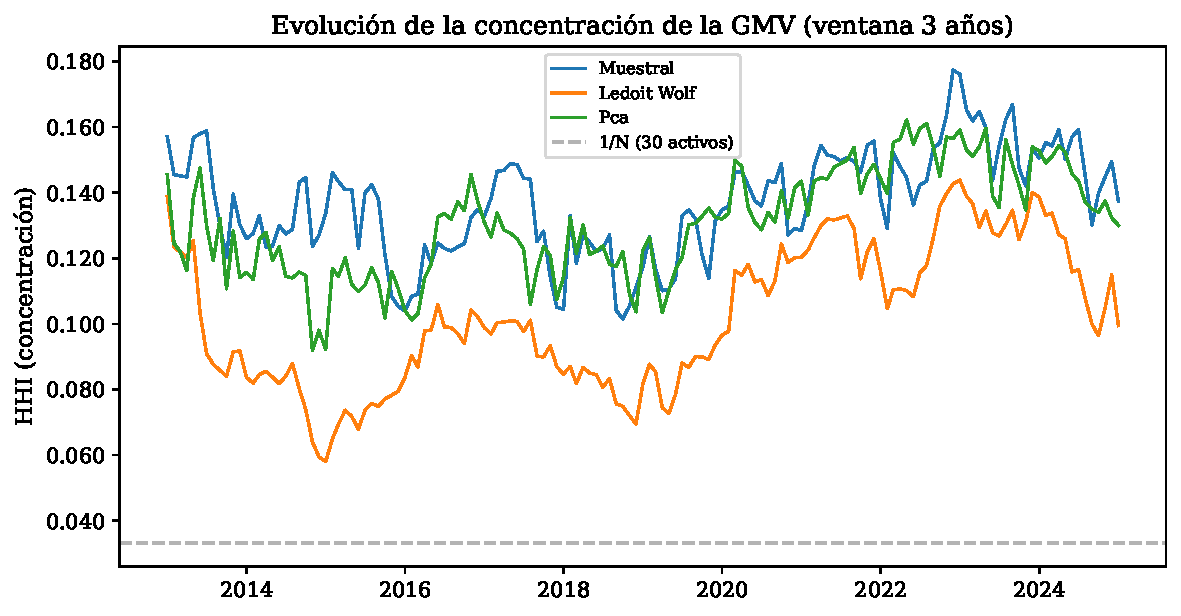
\includegraphics[width=0.60\textwidth]{../data/outputs/hhi_temporal}
    \caption{Evolución del índice Herfindahl-Hirschman (HHI) de la
             cartera GMV con ventanas móviles de 36 meses. La línea
             gris discontinua marca el HHI de la cartera equiponderada
             ($1/30 \approx 0{,}033$).}
    \label{fig:hhi-temporal}
\end{figure}

La inestabilidad de los pesos provoca dos problemas. El primero es un
\textbf{turnover} elevado: si los pesos óptimos cambian mucho de un mes a otro,
hay que comprar y vender activos con frecuencia, y esas comisiones reducen la
rentabilidad final. El segundo es la \textbf{concentración}: la cartera acaba
invertida en pocos activos, justo lo contrario de diversificar, y así asume el
riesgo particular de esos títulos, un riesgo que el mercado no remunera porque
podría haberse eliminado repartiendo mejor la inversión.

%--------------------------------------------------------------------
\section{Estimación robusta de la covarianza: shrinkage de Ledoit-Wolf}
\label{sec:ledoit-wolf}
%--------------------------------------------------------------------

\subsection{Fundamento teórico}

La idea del \textit{shrinkage} es sencilla: en lugar de fiarse por completo de
la matriz muestral (precisa en promedio, pero muy ruidosa), se mezcla con una
matriz simple y estable, y se toma un punto intermedio. Formalmente, el
\textit{shrinkage} es una técnica de regularización que contrae el estimador
muestral hacia un estimador estructurado (el \textit{target}), reduciendo el
error cuadrático medio esperado a cambio de introducir un pequeño sesgo. Ledoit
y Wolf \cite{Ledoit2004} propusieron un estimador de covarianza que es
combinación convexa (una media ponderada) del estimador muestral
$\boldsymbol{\Sigma}_{\text{muestral}}$ y un target
$\boldsymbol{\Sigma}_{\text{target}}$:
\begin{equation}
    \boldsymbol{\Sigma}_{\text{LW}} = (1 - \delta)\,
    \boldsymbol{\Sigma}_{\text{muestral}} + \delta\,
    \boldsymbol{\Sigma}_{\text{target}},
    \label{eq:ledoit-wolf}
\end{equation}
donde $\delta \in [0, 1]$ es la intensidad de shrinkage, calculada
analíticamente para minimizar el error cuadrático medio esperado
asintóticamente.

El target por defecto en \texttt{scikit-learn} (y en nuestra implementación) es
una \textbf{identidad escalada}: una matriz diagonal cuyos elementos valen todos
la varianza media de los activos, con correlaciones nulas fuera de la diagonal,
\begin{equation}
    [\boldsymbol{\Sigma}_{\text{target}}]_{ij} =
    \begin{cases}
        \bar{\sigma}^2 & \text{si } i = j, \\
        0 & \text{si } i \neq j,
    \end{cases}
    \qquad
    \bar{\sigma}^2 = \frac{1}{n}\sum_{k=1}^{n} \sigma_{kk}^{\text{muestral}}.
    \label{eq:target-lw}
\end{equation}
Es un target muy bien condicionado (todos sus autovalores valen
$\bar{\sigma}^2$), y al mezclarlo con la matriz muestral se atenúan los
autovalores extremos y las correlaciones espurias.

\subsection{Efecto sobre la cartera}

El efecto del shrinkage sobre los pesos de la cartera GMV se aprecia
en la Tabla~\ref{tab:comparativa-sigma}: la cartera Ledoit-Wolf es la
más diversificada de las tres. Esto se debe a que el shrinkage contrae
los autovalores hacia su media: baja los más grandes y, sobre todo, sube
los más pequeños, que son los que hacen inestable a
$\boldsymbol{\Sigma}^{-1}$ y los que el QP explotaría para concentrar
los pesos.

La Figura~\ref{fig:pesos-estimadores} compara visualmente la
distribución de pesos obtenida con cada estimador.

\begin{figure}[htbp]
    \centering
    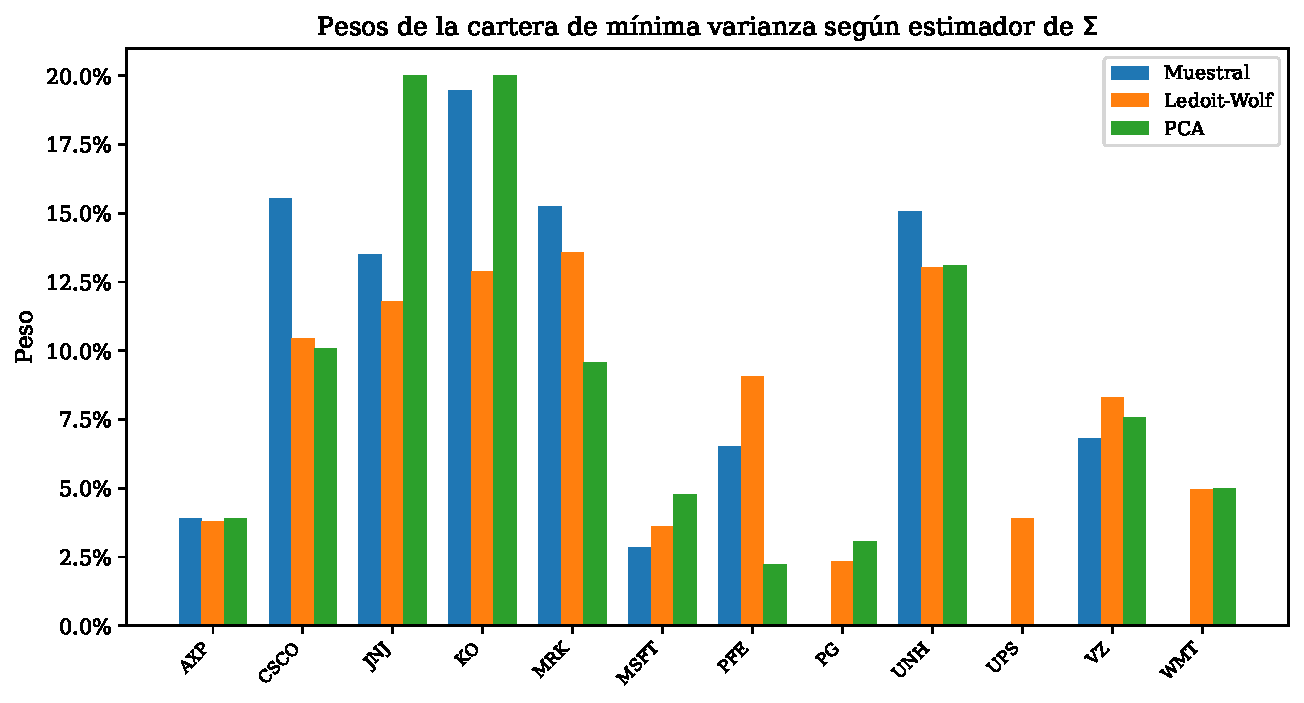
\includegraphics[width=0.66\textwidth]{../data/outputs/pesos_por_estimador}
    \caption{Pesos de la cartera GMV según el estimador de
             $\boldsymbol{\Sigma}$ (solo activos con peso $> 2\%$
             en al menos un estimador).}
    \label{fig:pesos-estimadores}
\end{figure}

%--------------------------------------------------------------------
\section{Covarianza basada en PCA y modelos de factores}
\label{sec:pca}
%--------------------------------------------------------------------

La idea es que casi todo lo que mueve a los activos a la vez se debe a unos
pocos factores comunes, como el mercado en su conjunto o los sectores; el PCA
identifica esos factores y separa esa estructura común del ruido propio de cada
activo. La matriz de covarianza muestral admite una descomposición espectral
$\boldsymbol{\Sigma} = \sum_{i=1}^{n} \lambda_i \mathbf{v}_i \mathbf{v}_i^T$,
con autovalores $\lambda_1 \ge \dots \ge \lambda_n \ge 0$, cada uno la varianza
explicada por su componente principal. El estimador PCA retiene solo los $k$
primeros componentes (los factores comunes), descarta el resto como ruido y
conserva la varianza específica de cada activo; su construcción detallada se
recoge en el Apéndice~\ref{ap:pca-apt}.

\subsection{Selección del número de factores}

La Figura~\ref{fig:scree-plot} muestra los autovalores de la matriz
de covarianza muestral y la varianza explicada acumulada para la
ventana 2022--2024.

\begin{figure}[htbp]
    \centering
    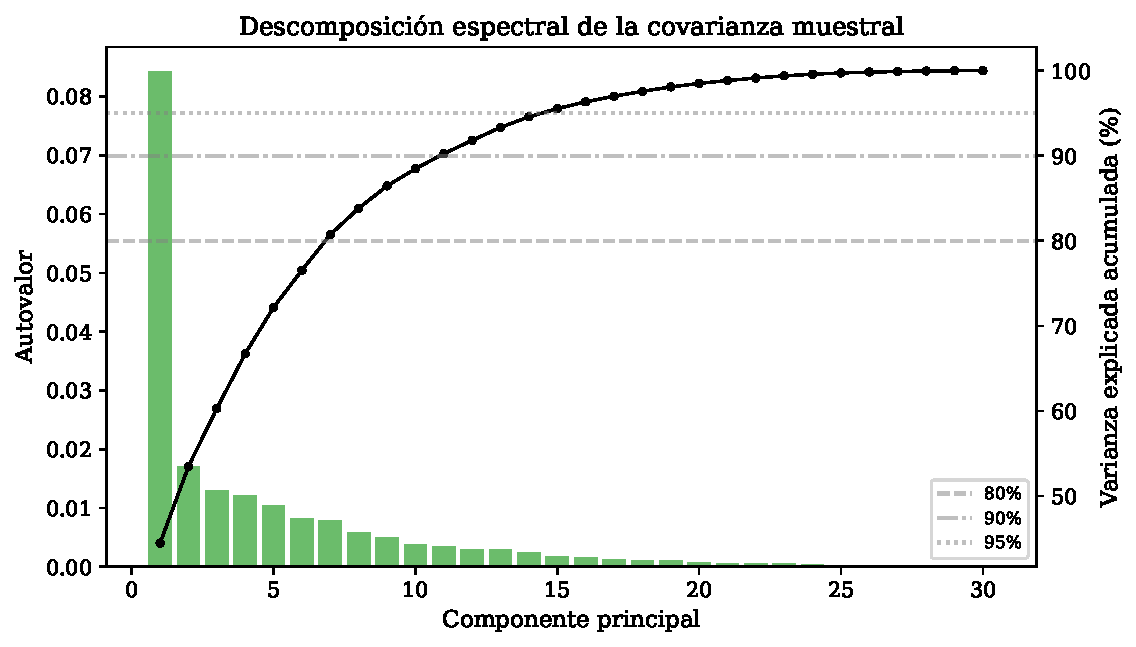
\includegraphics[width=0.55\textwidth]{../data/outputs/scree_plot}
    \caption{Descomposición espectral de la covarianza muestral.
             Barras: autovalores (eje izquierdo). Línea: varianza
             explicada acumulada (eje derecho).}
    \label{fig:scree-plot}
\end{figure}

El primer componente principal explica el 44,5\% de la varianza total;
con 7 componentes se alcanza el 80\% y con 11 componentes el 90\%.
Esto indica que la mayor parte de la variabilidad de las rentabilidades
de los 30 activos puede capturarse con un número reducido de factores
comunes, lo que justifica el uso de un modelo de factores para la
estimación de la covarianza.

\subsection{Conexión con la Arbitrage Pricing Theory (APT)}

La \textit{Arbitrage Pricing Theory} (APT) de Ross \cite{Ross1976} sostiene que
las rentabilidades de los activos dependen de unos pocos factores de riesgo
comunes y de una parte propia de cada activo. La conexión con lo anterior es
directa: si se toman como factores los $k$ primeros componentes principales, el
estimador PCA coincide exactamente con ese modelo de factores (la equivalencia
se demuestra en el Apéndice~\ref{ap:pca-apt}). Dicho de otro modo, los
componentes principales de la covarianza actúan como los factores de riesgo de
la teoría financiera. Esta correspondencia conecta el enfoque puramente
estadístico (la descomposición espectral) con la teoría financiera de factores,
y es uno de los puntos metodológicamente más relevantes de este trabajo.

%--------------------------------------------------------------------
\section{Síntesis: del error de estimación a la necesidad de Machine Learning}
%--------------------------------------------------------------------

La estimación de $\boldsymbol{\Sigma}$ puede mejorarse con regularización
(shrinkage) o reducción de dimensionalidad (PCA), pero la de
$\boldsymbol{\mu}$ sigue siendo el punto débil del modelo. De hecho, la
Tabla~\ref{tab:comparativa-sigma} muestra que los tres estimadores de
$\boldsymbol{\Sigma}$ dan volatilidades muy parecidas con pesos muy distintos:
la elección del estimador afecta más a la composición de la cartera que a su
riesgo ex-ante. La rentabilidad realizada, en cambio, depende sobre todo de
$\boldsymbol{\mu}$, el parámetro más difícil de estimar. De ahí que el
Capítulo~\ref{ch:ml} recurra al Machine Learning para predecirlo: si se estima
mejor $\boldsymbol{\mu}$, se puede aspirar a carteras con rentabilidad
out-of-sample superior a las estrategias pasivas de referencia.

\chapter{Machine Learning para la predicción de \texorpdfstring{$\boldsymbol{\mu}$}{μ}}
\label{ch:ml}

El Capítulo~\ref{ch:limitaciones} demostró que la estimación de
$\boldsymbol{\mu}$ es el punto más débil del modelo de Markowitz: la media
muestral tiene un error estándar comparable al propio parámetro, y ningún
estimador de $\boldsymbol{\Sigma}$ puede compensar una mala estimación de las
rentabilidades esperadas. Este capítulo explora si las técnicas de Machine
Learning pueden mejorar la estimación de $\boldsymbol{\mu}$ explotando
relaciones predecibles entre las características observables de los activos
y sus rentabilidades futuras.

%--------------------------------------------------------------------
\section{Planteamiento del problema predictivo}
%--------------------------------------------------------------------

\subsection{¿Por qué Machine Learning?}

La estimación tradicional de $\boldsymbol{\mu}$ como media histórica asume
implícitamente que las rentabilidades son independientes e idénticamente
distribuidas (i.i.d.). Si esta hipótesis fuera cierta, la media muestral sería
el mejor estimador lineal insesgado de $\mu_i$. Sin embargo, existe
abundante evidencia empírica de que las rentabilidades no son i.i.d.:
presentan \textbf{autocorrelación} a corto plazo (momentum, reversión a la
media), dependencia de la \textbf{volatilidad} (clustering) y sensibilidad a
\textbf{factores de riesgo} comunes \cite{Cont2001}.

Si existe una función $f$ que relaciona características observables
$\mathbf{x}_{i,t}$ del activo $i$ en el instante $t$ con su rentabilidad
futura $r_{i,t+1}$,
\begin{equation}
    r_{i,t+1} = f(\mathbf{x}_{i,t}) + \varepsilon_{i,t+1},
    \label{eq:ml-model}
\end{equation}
entonces un modelo de ML puede aproximar $f$ a partir de datos históricos,
produciendo una estimación de $\mu_{i,t+1} = \E[r_{i,t+1} \mid
\mathbf{x}_{i,t}]$ potencialmente más precisa que la media incondicional.

La clave está en que el modelo aprende de \textbf{todos los activos}
simultáneamente (o al menos comparte estructura entre ellos), lo que mitiga
la escasez de datos por activo: en lugar de estimar una media
por activo con 36 observaciones, el modelo estima una función $f$ con
$30 \times 36 = 1080$ observaciones, reduciendo la varianza del estimador.

\subsection{Configuración del problema}
\label{subsec:config-ml}

Para cada activo $i \in \{1, \dots, n\}$ y cada mes $t$, definimos:

\begin{itemize}
    \item \textbf{Target:} $y_{i,t} = r_{i,t+1}$, la rentabilidad logarítmica
          del activo $i$ en el mes $t+1$.
    \item \textbf{Features:} $\mathbf{x}_{i,t} \in \mathbb{R}^p$, un vector
          de $p$ características del activo $i$ calculadas exclusivamente con
          información disponible hasta el mes $t$ (inclusive).
\end{itemize}

El modelo se entrena de forma \textbf{agrupada} (\textit{pooled}): se estima una
única función $f$ común a todos los activos, apilando las observaciones de los
$n$ activos de la ventana. Así cada ajuste dispone de $n \times 36$
observaciones en lugar de 36, lo que reduce drásticamente la varianza del
estimador; las predicciones siguen siendo individualizadas porque cada activo
entra con sus propias features $\mathbf{x}_{i,t}$.

%--------------------------------------------------------------------
\section{Ingeniería de características (features)}
%--------------------------------------------------------------------

La selección de features está guiada por la literatura sobre predictibilidad
de rentabilidades \cite{Gu2020} y por la restricción fundamental de este
trabajo: solo se utilizan datos de precio (no fundamentales), ya que el
objetivo es un modelo puramente técnico que pueda automatizarse sin depender
de fuentes de datos externas.

\subsection{Features basadas en rentabilidades pasadas}

\begin{itemize}
    \item \textbf{Rezagos simples:} $r_{i,t}$, $r_{i,t-1}$, $r_{i,t-2}$.
          Capturan efectos de autocorrelación a muy corto plazo (reversión
          o continuación).
    \item \textbf{Momentum:} rentabilidad acumulada en los últimos 3, 6 y 12
          meses:
          \begin{equation}
              \text{mom}_{k}(i,t) = \sum_{j=0}^{k-1} r_{i,\,t-j},
              \quad k \in \{3, 6, 12\}.
              \label{eq:momentum}
          \end{equation}
          El momentum a 12 meses es uno de los factores más robustos en la
          literatura de \textit{cross-section} de rentabilidades
          \cite{Jegadeesh1993}.
    \item \textbf{Volatilidad realizada:} desviación típica de las
          rentabilidades de los últimos 12 meses, $\sigma_{i,t}^{(12)}$.
    \item \textbf{Beta al mercado:} pendiente de la regresión de $r_i$ sobre
          $r_m$ (SPY) en ventana de 36 meses,
          $\beta_{i,t} = \Cov_{36\text{m}}(r_i, r_m)/\Var_{36\text{m}}(r_m)$.
\end{itemize}

\subsection{Features del mercado}

Además de las características propias de cada activo, se incluyen features
que capturan el contexto de mercado:
\begin{itemize}
    \item \textbf{Rezagos del mercado:} $r_{m,t}$, $r_{m,t-1}$ (rentabilidad
          del SPY).
    \item \textbf{Volatilidad del mercado:} $\sigma_{m,t}^{(12)}$, desviación
          típica del SPY en 12 meses.
\end{itemize}

En total, el vector de features tiene dimensión $p = 11$. La
Tabla~\ref{tab:features} resume las features utilizadas.

\begin{table}[htbp]
    \centering
    \caption{Features utilizadas para la predicción de $r_{i,t+1}$.}
    \label{tab:features}
    \begin{tabular}{ll}
        \toprule
        \textbf{Feature} & \textbf{Descripción} \\
        \midrule
        \texttt{r\_lag1}, \texttt{r\_lag2}, \texttt{r\_lag3} & Rezagos del activo ($t$, $t-1$, $t-2$) \\
        \texttt{mom3}, \texttt{mom6}, \texttt{mom12} & Momentum a 3, 6 y 12 meses \\
        \texttt{vol12} & Volatilidad realizada a 12 meses \\
        \texttt{beta\_36m} & Beta rolling al SPY (36 meses) \\
        \texttt{r\_mkt\_lag1}, \texttt{r\_mkt\_lag2} & Rezagos del SPY \\
        \texttt{r\_mkt\_vol12} & Volatilidad del SPY a 12 meses \\
        \bottomrule
    \end{tabular}
\end{table}

%--------------------------------------------------------------------
\section{Modelos de Machine Learning}
%--------------------------------------------------------------------

Se implementan tres modelos que representan distintos compromisos entre sesgo
y varianza, flexibilidad e interpretabilidad.

\subsection{Ridge (regularización L2)}

Ridge \cite{HoerlKennard1970} es una regresión lineal con penalización en la
norma $\ell_2$ de los coeficientes:
\begin{equation}
    \hat{\boldsymbol{\beta}}_{\text{Ridge}} =
    \arg\min_{\boldsymbol{\beta}} \left\{
    \sum_{i,t} (y_{i,t} - \mathbf{x}_{i,t}^T \boldsymbol{\beta})^2
    + \alpha \sum_{j=1}^{p} \beta_j^2
    \right\},
    \label{eq:ridge}
\end{equation}
donde la primera suma recorre las observaciones apiladas de todos los activos
(la muestra agrupada de la Sección~\ref{subsec:config-ml}).

La penalización $\ell_2$ contrae los coeficientes hacia cero sin anularlos:
reduce la varianza del estimador a cambio de un pequeño sesgo, y es adecuada
cuando muchas features tienen poder predictivo débil pero no nulo o están muy
correlacionadas entre sí. En ese caso, una regresión sin penalizar daría
coeficientes muy grandes e inestables (la matriz $\mathbf{X}^T\mathbf{X}$ queda
mal condicionada, casi singular); la penalización de Ridge los estabiliza. El
hiperparámetro $\alpha$ ---de $0$ (mínimos cuadrados ordinarios) a $\infty$
(todos los coeficientes nulos)--- se selecciona por validación cruzada temporal
(\textit{TimeSeriesSplit}) en 10 valores entre $10^{-3}$ y $10^{2}$. Como el
entrenamiento es agrupado sobre activos de escalas heterogéneas, las features se
estandarizan (media 0, varianza 1) usando solo la muestra de entrenamiento.

\subsection{Lasso (regularización L1)}

Lasso \cite{Tibshirani1996} sustituye la penalización $\ell_2$ por $\ell_1$:
\begin{equation}
    \hat{\boldsymbol{\beta}}_{\text{Lasso}} =
    \arg\min_{\boldsymbol{\beta}} \left\{
    \sum_{i,t} (y_{i,t} - \mathbf{x}_{i,t}^T \boldsymbol{\beta})^2
    + \alpha \sum_{j=1}^{p} |\beta_j|
    \right\}.
    \label{eq:lasso}
\end{equation}

La norma $\ell_1$ produce soluciones \textbf{sparse} (muchos coeficientes
exactamente cero): Lasso hace selección automática de features y es más
interpretable que Ridge, a costa de más inestabilidad con features muy
correlacionadas \cite{Zou2005}. Como en Ridge, las features se estandarizan y
$\alpha$ se elige por validación cruzada temporal en el mismo rango.

\subsection{Random Forest}

Random Forest es un método no paramétrico basado en un \textit{ensemble} de
árboles de decisión \cite{Breiman2001}. Cada árbol particiona recursivamente
el espacio de features para minimizar el error cuadrático medio en cada nodo,
y el bosque promedia las predicciones de todos los árboles.

Sus principales ventajas aquí son que captura relaciones no lineales e
interacciones entre features sin especificarlas, es robusto a outliers y a
features irrelevantes, y el promediado sobre muchos árboles (100 en la
implementación) reduce la varianza sin aumentar el sesgo.

Para evitar el sobreajuste se limitan la profundidad máxima de cada árbol a 3
y el número mínimo de muestras por hoja a 5. Estos hiperparámetros, junto con
el número de árboles (100), se mantienen fijos para todo el backtesting. A
diferencia de los modelos lineales, Random Forest no requiere estandarizar las
features, al ser invariante a transformaciones monótonas de cada variable.

%--------------------------------------------------------------------
\section{Validación temporal (walk-forward)}
%--------------------------------------------------------------------

\subsection{El peligro del look-ahead}

En la predicción de series temporales financieras, la validación cruzada
estándar (aleatoria) es metodológicamente incorrecta: al barajar las
observaciones, se rompe la estructura temporal y el modelo podría entrenarse
con datos del futuro para predecir el pasado. Esto produce estimaciones
irrealmente optimistas del rendimiento predictivo y, lo que es más grave,
contamina la selección de hiperparámetros.

Por esta razón, toda la validación se realiza en régimen walk-forward:
en cada mes $t$, el modelo solo puede acceder a datos hasta $t$ para
entrenar, validar hiperparámetros y predecir.

\subsection{Protocolo de backtesting}

En cada mes $t$, el modelo se entrena solo con datos hasta $t$ (ventana de 36
meses), predice $\hat{\mu}_{i,t+1}$ para cada activo a partir de sus features de
$t$, y esas predicciones ---junto con $\hat{\boldsymbol{\Sigma}}$--- alimentan la
optimización de la cartera de máximo Sharpe, cuya rentabilidad se evalúa en
$t+1$. El ciclo se repite 143 veces (enero 2013 -- diciembre 2024). El
Capítulo~\ref{ch:metodologia} detalla el protocolo completo y las medidas que
se toman para evitar el look-ahead.

\subsection{Métricas de evaluación predictiva}

Para evaluar la calidad de las predicciones de $\boldsymbol{\mu}$, se calculan
las siguientes métricas sobre las predicciones out-of-sample de cada modelo:

\begin{itemize}
    \item \textbf{RMSE} (Root Mean Square Error):
          $\sqrt{\frac{1}{nT} \sum_{i,t} (r_{i,t+1} - \hat{\mu}_{i,t})^2}$.
    \item \textbf{MAE} (Mean Absolute Error):
          $\frac{1}{nT} \sum_{i,t} |r_{i,t+1} - \hat{\mu}_{i,t}|$.
    \item \textbf{$R^2$ out-of-sample}:
          $1 - \frac{\sum_{i,t} (r_{i,t+1} - \hat{\mu}_{i,t})^2}
          {\sum_{i,t} (r_{i,t+1} - \bar{r})^2}$,
          donde $\bar{r}$ es la media histórica. Un $R^2$ positivo indica que
          el modelo ML mejora sobre la media histórica.
    \item \textbf{Correlación de Pearson} entre $\hat{\boldsymbol{\mu}}$ y
          $\mathbf{r}_{t+1}$ realizada, agregada a nivel de mes.
\end{itemize}

En finanzas, incluso un $R^2$ pequeño
($\approx 0{,}01$--$0{,}05$) puede ser económicamente significativo si se
traduce en una mejora del ratio de Sharpe de la cartera optimizada.

%--------------------------------------------------------------------
\section{Conexión con la optimización de carteras}
%--------------------------------------------------------------------

El objetivo no es minimizar el RMSE de
$\hat{\boldsymbol{\mu}}$, sino maximizar el rendimiento out-of-sample de la
cartera: un RMSE bajo no garantiza una buena cartera, y el QP puede
beneficiarse más de acertar el \textit{orden} (ranking) de los activos que de
minimizar el error cuadrático. Por eso la evaluación definitiva se hace sobre
las métricas de cartera (Sharpe, drawdown, turnover) del
Capítulo~\ref{ch:resultados}, y las predictivas se reportan solo como
diagnóstico complementario.

%--------------------------------------------------------------------
\section{Síntesis}

En resumen, este capítulo aborda la principal limitación del modelo clásico
---la estimación de $\boldsymbol{\mu}$--- con un marco de Machine Learning que
usa 11 features exclusivamente de precio, tres modelos complementarios (Ridge,
Lasso y Random Forest), una validación temporal estricta sin look-ahead y, como
métrica final, el rendimiento de la cartera y no el RMSE de la predicción. El
Capítulo~\ref{ch:metodologia} detalla cómo se integran estos modelos con los
estimadores de covarianza del Capítulo~\ref{ch:limitaciones} en el backtesting
walk-forward.

\chapter{Metodología y diseño experimental}
\label{ch:metodologia}

Este capítulo describe la metodología completa del estudio: los datos
utilizados, el esquema de backtesting walk-forward, las carteras evaluadas
y las métricas de rendimiento. El objetivo es que el experimento sea
completamente reproducible con los datos y el código proporcionados.

%--------------------------------------------------------------------
\section{Datos}
%--------------------------------------------------------------------

\subsection{Universo de activos}

El universo de inversión está compuesto por 30 acciones del S\&P 500,
seleccionadas de modo que cubren los once sectores GICS. La
Tabla~\ref{tab:universo} detalla los tickers y sus sectores.

\begin{table}[htbp]
    \centering
    \caption{Universo de 30 activos por sector GICS.}
    \label{tab:universo}
    \begin{tabular}{ll}
        \toprule
        \textbf{Sector} & \textbf{Tickers} \\
        \midrule
        Tecnología & AAPL, MSFT, ORCL, CSCO, INTC \\
        Salud & JNJ, PFE, MRK, UNH \\
        Finanzas & JPM, GS, AXP, BAC \\
        Consumo discrecional & HD, MCD, NKE \\
        Consumo básico & PG, KO, WMT \\
        Comunicaciones & VZ, T, DIS \\
        Energía & XOM, CVX \\
        Industriales & CAT, HON, UPS \\
        Materiales & FCX \\
        Utilities & NEE \\
        Inmobiliario & AMT \\
        \bottomrule
    \end{tabular}
\end{table}

Como referencia de mercado se utiliza el \textbf{SPY} (SPDR S\&P 500 ETF
Trust), que replica el S\&P 500 y no forma parte del universo a optimizar.

\subsection{Periodo y frecuencia}

\begin{itemize}
    \item \textbf{Periodo total:} 1 de enero de 2010 -- 31 de diciembre de
          2024 (15 años).
    \item \textbf{Datos diarios:} 3.773 días de negociación para 31 tickers
          (30 acciones + SPY).
    \item \textbf{Frecuencia de trabajo:} mensual. Los retornos logarítmicos
          diarios se agregan a frecuencia mensual mediante suma:
          $r_t^{\text{mensual}} = \sum_{d \in \text{mes}(t)} r_d^{\text{diaria}}$,
          propiedad que deriva de la aditividad de los log-retornos
          (ecuación~\ref{eq:aditividad-log}).
    \item \textbf{Meses resultantes:} 180 meses (enero 2010 -- diciembre 2024).
\end{itemize}

\subsection{Fuente y preprocesado}

Los precios ajustados (cierre) se descargan de \textbf{Yahoo Finance} a
través de la librería \texttt{yfinance} de Python. El preprocesado consiste en:

\begin{enumerate}
    \item \textbf{Cálculo de retornos logarítmicos diarios:}
          $r_t = \ln(P_t / P_{t-1})$.
    \item \textbf{Limpieza:} eliminación de días sin negociación,
          \textit{forward-fill} de datos faltantes.
    \item \textbf{Agregación mensual:} suma de retornos diarios dentro de
          cada mes natural.
\end{enumerate}

Se reconoce explícitamente la presencia de \textbf{sesgo de supervivencia}:
el universo está compuesto por constituyentes actuales (2024) del S\&P 500,
no por los constituyentes históricos. Esto implica que las empresas que
quebraron o fueron excluidas del índice durante el periodo de estudio no
están representadas. El sesgo tiende a sobreestimar ligeramente las
rentabilidades históricas, pero su impacto en un estudio de asignación de
activos como este es limitado, ya que el objetivo es comparar metodologías
de optimización, no estimar rentabilidades absolutas.

%--------------------------------------------------------------------
\section{Esquema de backtesting walk-forward}
%--------------------------------------------------------------------

El experimento sigue un protocolo de backtesting walk-forward con
rebalanceo mensual, que constituye el estándar metodológico en la literatura
de optimización de carteras \cite{DeMiguel2009}.

\subsection{Parámetros del backtesting}

\begin{itemize}
    \item \textbf{Ventana de estimación:} 36 meses (3 años).
    \item \textbf{Frecuencia de rebalanceo:} mensual.
    \item \textbf{Periodo out-of-sample:} enero 2013 -- diciembre 2024
          (144 meses, de los cuales se evalúan 143 por el desfase de la
          predicción).
    \item \textbf{Restricciones:} long-only ($w_i \ge 0$), peso máximo por
          activo $w_i \le 0{,}20$, presupuesto $\sum_i w_i = 1$.
\end{itemize}

\subsection{Procedimiento mensual}

Para cada mes $t$ desde enero de 2013 ($t = 37$) hasta noviembre de 2024
($t = 179$): se toma la ventana de 36 meses ($t-35, \dots, t$); se estima
$\boldsymbol{\Sigma}$ con uno de los tres estimadores (muestral, Ledoit-Wolf o
PCA al 80\% de varianza) y $\boldsymbol{\mu}$ con uno de los cuatro métodos
(media histórica, Ridge, Lasso o RF); se resuelve el QP de mínimo riesgo
(ecuación~\ref{eq:qp-riesgo}) barriendo el objetivo de rentabilidad $\mu^*$ y
se toma el punto de
máximo Sharpe, que da los pesos $\mathbf{w}_t$; y se evalúa la rentabilidad
realizada $r_{p,t+1} = \mathbf{w}_t^T \mathbf{r}_{t+1}$.

Esquemáticamente, para un total de $T=180$ meses:
\[
\underbrace{r_2, \dots, r_{37}}_{\text{Train}_1} \to
\underbrace{r_{38}}_{\text{Pred}_1} \quad
\underbrace{r_3, \dots, r_{38}}_{\text{Train}_2} \to
\underbrace{r_{39}}_{\text{Pred}_2} \quad
\cdots \quad
\underbrace{r_{144}, \dots, r_{179}}_{\text{Train}_{143}} \to
\underbrace{r_{180}}_{\text{Pred}_{143}}
\]

donde Train$_k$ es la ventana de 36 meses usada para estimar
$\boldsymbol{\mu}$ y $\boldsymbol{\Sigma}$ en la iteración $k$, y Pred$_k$
es el mes out-of-sample cuya rentabilidad $r_{p,k}$ se evalúa.

\subsection{Prevención del look-ahead}

Para evitar el look-ahead se toman las siguientes medidas:
\begin{itemize}
    \item La estimación de $\boldsymbol{\Sigma}$ en el mes $t$ solo utiliza
          rentabilidades hasta $t$.
    \item Las features para la predicción ML en $t$ solo utilizan datos
          hasta $t$ (ver Capítulo~\ref{ch:ml}).
    \item La rentabilidad out-of-sample $r_{p,t+1}$ \textbf{no} se utiliza
          en ningún paso de la optimización para el mes $t$.
    \item La validación cruzada para la selección de hiperparámetros de los
          modelos ML se realiza con \texttt{TimeSeriesSplit}, que respeta el
          orden cronológico.
\end{itemize}

%--------------------------------------------------------------------
\section{Carteras evaluadas}
%--------------------------------------------------------------------

Se evalúan 8 carteras, presentadas en la Tabla~\ref{tab:carteras-evaluadas}.
Las tres primeras corresponden al modelo de Markowitz clásico con distintos
estimadores de $\boldsymbol{\Sigma}$, las tres siguientes incorporan
predicciones ML de $\boldsymbol{\mu}$, y las dos últimas son baselines
pasivos.

\begin{table}[htbp]
    \centering
    \caption{Carteras evaluadas en el experimento.}
    \label{tab:carteras-evaluadas}
    \begin{tabular}{lll}
        \toprule
        \textbf{Cartera} & \textbf{Estimador de $\boldsymbol{\Sigma}$} & \textbf{Estimador de $\boldsymbol{\mu}$} \\
        \midrule
        Markowitz (muestral) & Muestral & Media histórica \\
        Markowitz (Ledoit-Wolf) & Ledoit-Wolf & Media histórica \\
        Markowitz (PCA) & PCA (80\% var.) & Media histórica \\
        Markowitz + Ridge & Ledoit-Wolf & Ridge \\
        Markowitz + Lasso & Ledoit-Wolf & Lasso \\
        Markowitz + RF & Ledoit-Wolf & Random Forest \\
        1/N (equiponderada) & -- & -- \\
        SPY (mercado) & -- & -- \\
        \bottomrule
    \end{tabular}
\end{table}

\textbf{Nota sobre la elección de $\boldsymbol{\Sigma}$ para las estrategias
ML:} se utiliza el estimador de Ledoit-Wolf para todas ellas, por ser el más
fiable en términos de diversificación y estabilidad
(Capítulo~\ref{ch:limitaciones}). Esto permite aislar el efecto de la mejora
en $\boldsymbol{\mu}$ sin que las diferencias en $\boldsymbol{\Sigma}$
contaminen la comparación.

%--------------------------------------------------------------------
\section{Métricas de evaluación}
%--------------------------------------------------------------------

\subsection{Métricas de rentabilidad-riesgo}

Sobre la serie de 143 rentabilidades mensuales out-of-sample de cada
cartera, se calculan:

\begin{itemize}
    \item \textbf{Rentabilidad anualizada} (compuesta geométricamente):
          \begin{equation}
              r_{\text{anual}} = \Bigl(\prod_{t=1}^{T} (1 + r_{p,t})
              \Bigr)^{12/T} - 1.
              \label{eq:rent-anual}
          \end{equation}
    \item \textbf{Volatilidad anualizada:}
          $\sigma_{\text{anual}} = \sigma_{\text{mensual}} \cdot \sqrt{12}$.
    \item \textbf{Ratio de Sharpe} (anualizado, $r_f = 0$):
          $S_p = r_{\text{anual}} / \sigma_{\text{anual}}$.
    \item \textbf{Máximo drawdown:} máxima caída desde un pico anterior en la
          curva de valor acumulado. Expresado como:
          \begin{equation}
              \text{MDD} = \max_{t} \left(
              1 - \frac{V_t}{\max_{s \le t} V_s}
              \right),
              \label{eq:mdd}
          \end{equation}
          donde $V_t = \prod_{s=1}^{t} (1 + r_{p,s})$ es el valor acumulado
          de la cartera en el mes $t$.
\end{itemize}

\subsection{Métricas de composición de cartera}

\begin{itemize}
    \item \textbf{Turnover medio:} mide la rotación de la cartera entre
          rebalanceos consecutivos,
          \begin{equation}
              \text{TO} = \frac{1}{2(T-1)} \sum_{t=2}^{T}
              \sum_{i=1}^{n} |w_{i,t} - w_{i,t-1}|.
              \label{eq:turnover}
          \end{equation}
          El factor $1/2$ normaliza el turnover entre 0 (cartera estática)
          y 1 (rotación completa). Un turnover elevado implica mayores costes
          de transacción.
    \item \textbf{Índice Herfindahl-Hirschman (HHI) medio:}
          $\text{HHI} = \frac{1}{T} \sum_t \sum_i w_{i,t}^2$.
          Mide la concentración de la cartera: $1/n$ para la equiponderada,
          $1$ para un solo activo.
    \item \textbf{Número medio de activos en cartera:} media del número de
          activos con peso $> 0{,}1\%$ en cada rebalanceo.
\end{itemize}

\subsection{Métricas de predicción ML}

Para los modelos de ML se reportan además el RMSE, el MAE y el $R^2$
out-of-sample de las predicciones de $\boldsymbol{\mu}$ (definidos en el
Capítulo~\ref{ch:ml}); un $R^2$ negativo indica que el modelo predice peor que
la media histórica, aunque la cartera podría aun así mejorar a la clásica si
acierta el orden (ranking) de los activos.

%--------------------------------------------------------------------
\section{Implementación y reproducibilidad}
%--------------------------------------------------------------------

El código está implementado en Python 3.13 y organizado en módulos
independientes bajo \texttt{src/}:

\begin{itemize}
    \item \texttt{data\_ingest/}: descarga y preprocesado de datos.
    \item \texttt{optimization/}: optimización QP (\texttt{cvxpy}),
          estimación de covarianza (\texttt{scikit-learn}) y restricciones.
    \item \texttt{ml/}: feature engineering, modelos (Ridge, Lasso, RF) y
          pipeline de predicción.
    \item \texttt{backtest/}: motor de backtesting walk-forward y métricas
          de evaluación.
\end{itemize}

La carpeta \texttt{tests/} contiene los tests que validan la implementación:
la coincidencia de la solución numérica del QP con la solución analítica y el
cumplimiento de las condiciones KKT (Capítulo~\ref{ch:formulacion}). Se incluye
además, en \texttt{demo/}, una demostración web interactiva del optimizador,
como material de apoyo a la presentación del trabajo.

La reproducibilidad está garantizada mediante:
\begin{itemize}
    \item Semilla fija (\texttt{seed = 42}) para todos los componentes
          aleatorios.
    \item Versiones de dependencias congeladas en \texttt{requirements.txt}.
    \item Datos descargables automáticamente desde Yahoo Finance.
    \item Scripts de ejecución en \texttt{scripts/} que generan todas las
          tablas y figuras de la memoria.
\end{itemize}

%--------------------------------------------------------------------
\section{Síntesis}

El diseño experimental combina 6 carteras optimizadas (tres clásicas, una por
estimador de $\boldsymbol{\Sigma}$, y tres con $\boldsymbol{\mu}$ predicho por
ML sobre Ledoit-Wolf) y 2 baselines pasivos, un backtesting walk-forward de 143 meses out-of-sample (ventanas de 36
meses, rebalanceo mensual) y métricas de rentabilidad-riesgo, composición y
calidad predictiva. El Capítulo~\ref{ch:resultados} presenta los resultados y
el Capítulo~\ref{ch:conclusiones}, las conclusiones.

\chapter{Resultados y discusión}
\label{ch:resultados}

Este capítulo presenta y analiza los resultados del experimento descrito en
el Capítulo~\ref{ch:metodologia}. Se evalúan 6 carteras optimizadas (tres
clásicas, una por estimador de $\boldsymbol{\Sigma}$, y tres con
$\boldsymbol{\mu}$ predicho por ML) y 2 baselines pasivos sobre 143 meses
out-of-sample (enero 2013 -- diciembre 2024).

%--------------------------------------------------------------------
\section{Comparación global de carteras}
%--------------------------------------------------------------------

La Tabla~\ref{tab:resultados-globales} presenta las métricas de todas las
carteras evaluadas. La Figura~\ref{fig:sharpe-comparacion} ordena las
estrategias por ratio de Sharpe y la Figura~\ref{fig:valor-acumulado}
muestra la evolución del valor acumulado de 1\texteuro{} invertido.

\begin{table}[htbp]
    \centering
    \caption{Resultados completos del backtesting walk-forward
             (enero 2013 -- diciembre 2024, 143 meses).}
    \label{tab:resultados-globales}
    \resizebox{\textwidth}{!}{\begin{tabular}{lrrrrrrr}
\toprule
Estrategia & Rent. anual (\%) & Vol. anual (\%) & Sharpe & Máx. DD (\%) & Turnover & HHI & Nº activos \\
\midrule
Markowitz (muestral) & 8,34 & 12,97 & 0,64 & 32,26 & 0,14 & 0,15 & 8,85 \\
Markowitz (Ledoit-Wolf) & 8,86 & 12,99 & 0,68 & 29,30 & 0,13 & 0,14 & 10,62 \\
Markowitz (PCA) & 9,00 & 13,01 & 0,69 & 30,91 & 0,14 & 0,16 & 8,57 \\
Markowitz + Ridge & 9,29 & 13,72 & 0,68 & 18,42 & 0,57 & 0,14 & 11,17 \\
Markowitz + Lasso & 9,65 & 12,79 & 0,75 & 25,55 & 0,12 & 0,10 & 14,89 \\
Markowitz + RF & 9,84 & 13,91 & 0,71 & 24,09 & 0,36 & 0,12 & 13,62 \\
1/N (equiponderada) & 10,68 & 14,14 & 0,76 & 21,89 & 0,00 & 0,03 & 30,00 \\
SPY (mercado) & 12,94 & 14,42 & 0,90 & 25,48 & 0,00 & 1,00 & 1,00 \\
\bottomrule
\end{tabular}
}
\end{table}

\begin{figure}[htbp]
    \centering
    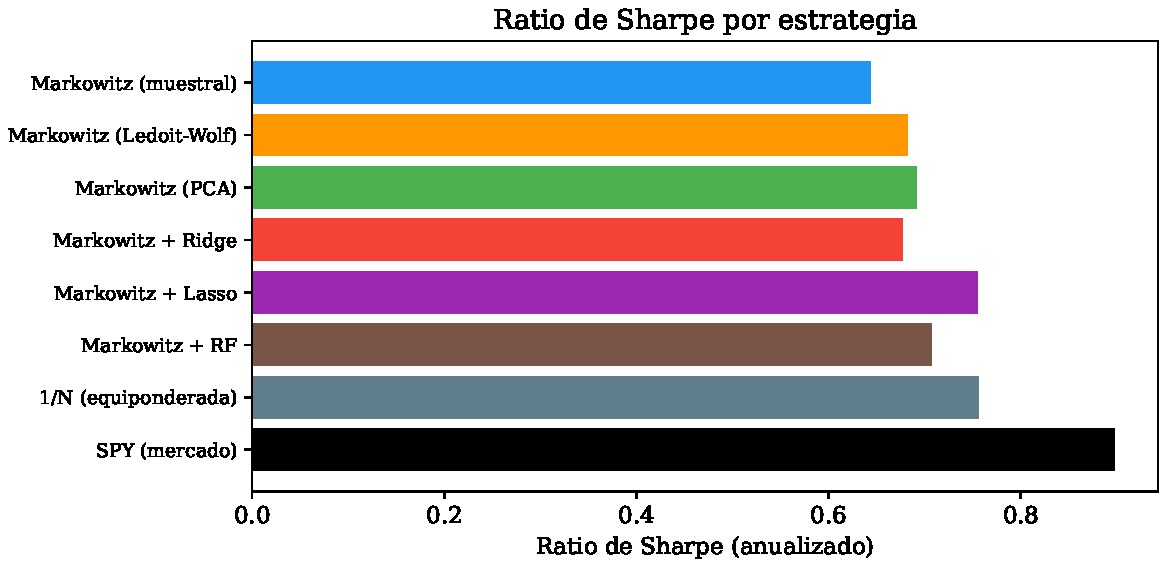
\includegraphics[width=0.56\textwidth]{../data/outputs/sharpe_comparacion}
    \caption{Ratio de Sharpe anualizado por estrategia.}
    \label{fig:sharpe-comparacion}
\end{figure}

\begin{figure}[htbp]
    \centering
    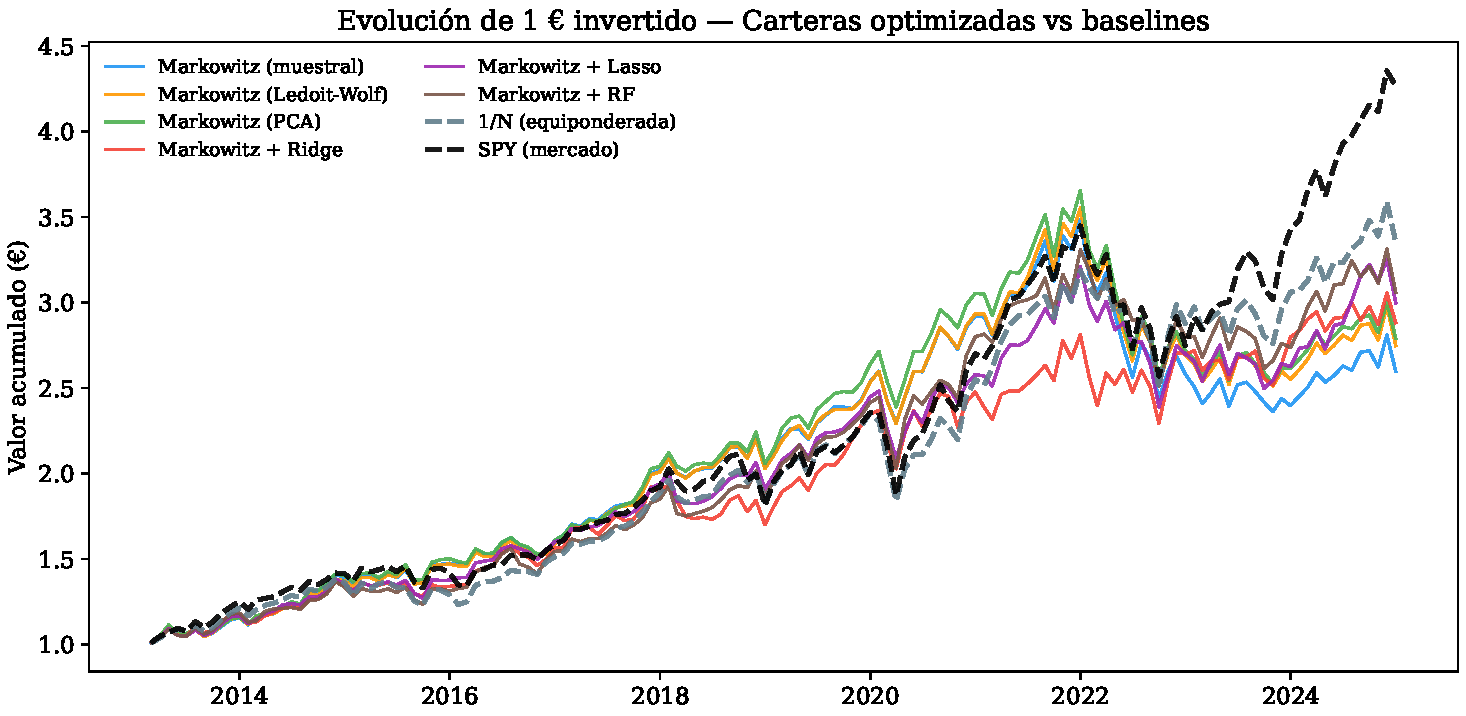
\includegraphics[width=0.66\textwidth]{../data/outputs/valor_acumulado}
    \caption{Evolución de 1\texteuro{} invertido en cada estrategia
             durante el periodo out-of-sample (2013--2024). Las líneas
             discontinuas representan los baselines pasivos.}
    \label{fig:valor-acumulado}
\end{figure}

\subsection{Resultado principal}

El hallazgo más relevante es que \textbf{ninguna cartera optimizada supera
a los baselines pasivos} en ratio de Sharpe. El SPY obtiene un Sharpe de
$0{,}90$ con una rentabilidad anualizada del $12{,}9\%$, y la cartera
$1/N$ equiponderada alcanza un Sharpe de $0{,}76$ con un $10{,}7\%$
anualizado.

Entre las carteras optimizadas, la \textbf{Markowitz + Lasso} es la mejor,
con un Sharpe de $0{,}75$ y una rentabilidad del $9{,}7\%$ anualizado, hasta
el punto de \emph{igualar} en la práctica a la cartera $1/N$ ($0{,}76$).
Le siguen \textbf{Markowitz + RF} (Sharpe $0{,}71$) y \textbf{Markowitz (PCA)}
($0{,}69$). No obstante, como se demuestra en la
Sección~\ref{sec:significancia}, ninguna de estas diferencias es
estadísticamente significativa.

Este resultado es consistente con la literatura: DeMiguel, Garlappi y Uppal
\cite{DeMiguel2009} demostraron que se necesitan ventanas de estimación
extremadamente largas (más de 3.000 meses) para que las carteras optimizadas
superen consistentemente a la $1/N$. Con 36 meses de ventana, el error de
estimación domina cualquier ganancia teórica de la optimización.

\subsection{Rentabilidad frente a riesgo}

Todas las carteras optimizadas presentan volatilidades muy similares
(12,8\%--13,9\% anual), cercanas a las de los baselines (14,1\%--14,4\%).
La diferencia está en la rentabilidad: el SPY genera un $12{,}9\%$ frente
al $8{,}3\%$--$9{,}8\%$ de las carteras optimizadas. Esto sugiere que el
principal lastre de las carteras optimizadas no es un exceso de riesgo,
sino una \textbf{rentabilidad sistemáticamente menor}: los activos que
selecciona el optimizador rinden, fuera de muestra, menos que el mercado.

%--------------------------------------------------------------------
\section{Efecto del estimador de covarianza}
%--------------------------------------------------------------------

La Tabla~\ref{tab:resultados-globales} permite comparar el efecto de los
tres estimadores de $\boldsymbol{\Sigma}$ cuando $\boldsymbol{\mu}$ se
estima como media histórica.

El estimador \textbf{muestral} es el peor (Sharpe $0{,}64$), con la mayor
concentración (HHI $0{,}15$; $8{,}9$ activos). \textbf{Ledoit-Wolf} lo mejora en
$+0{,}04$ ($0{,}68$), reduce la concentración (HHI $0{,}14$; $10{,}6$ activos) y
baja el drawdown ($29{,}3\%$ frente a $32{,}3\%$). \textbf{PCA} logra el mejor
Sharpe clásico ($0{,}69$), algo más rentable pero más concentrado (HHI $0{,}16$;
$8{,}6$ activos).

Esto confirma el análisis del Capítulo~\ref{ch:limitaciones}: Ledoit-Wolf da
las carteras más diversificadas y estables y el estimador muestral es el más
vulnerable al error de estimación, con PCA en una posición intermedia ---mejor
rentabilidad, pero menor diversificación.

%--------------------------------------------------------------------
\section{Efecto de la predicción ML de \texorpdfstring{$\boldsymbol{\mu}$}{μ}}
%--------------------------------------------------------------------

\subsection{Rendimiento de las carteras ML}

Las tres estrategias ML utilizan el estimador de covarianza Ledoit-Wolf y
se diferencian únicamente en el modelo de predicción de $\boldsymbol{\mu}$:

\begin{itemize}
    \item \textbf{Lasso} (Sharpe $0{,}75$) es la \textbf{mejor cartera
          optimizada} y prácticamente iguala a la $1/N$, con el menor turnover
          ($0{,}12$) y la mayor diversificación de las carteras optimizadas
          (14,9 activos, HHI $0{,}10$).
    \item \textbf{Random Forest} ($0{,}71$), el único modelo no lineal, queda
          en segundo lugar, con un turnover moderado ($0{,}36$).
    \item \textbf{Ridge} ($0{,}68$) se queda en el Sharpe del clásico de
          Ledoit-Wolf, pero logra el \textbf{menor drawdown del estudio}
          ($18{,}4\%$).
\end{itemize}

\subsection{Análisis del rendimiento de los modelos ML}

El factor decisivo es el \textbf{tamaño efectivo de la muestra de
entrenamiento}. Al estimar un único modelo agrupado sobre todos los activos
(Capítulo~\ref{ch:ml}), cada ajuste dispone de unas $30 \times 36 \approx 1.000$
observaciones en lugar de 36. Por eso incluso Random Forest se comporta de forma
estable (Sharpe $0{,}71$): con solo 36 observaciones por activo un modelo no
lineal sobreajustaría el ruido, pero con la muestra agrupada extrae una señal
débil pero consistente.

Entre los lineales, Lasso supera a Ridge: la regularización $\ell_1$ anula los
coeficientes sin poder predictivo (selección automática) y, en un entorno de muy
baja señal-ruido, produce predicciones parsimoniosas y estables ---de ahí el
bajísimo turnover de Lasso. De hecho, en muchos meses la validación cruzada elige
un nivel que anula todos los coeficientes y reduce $\hat{\boldsymbol{\mu}}$ a una
constante: cuando los datos no contienen señal aprovechable, el modelo lo
refleja tal cual, en lugar de forzar una predicción ruidosa. Todo ello es coherente con la literatura \cite{Gu2020}, que
subraya compartir información entre activos y regularizar con fuerza cuando los
datos escasean.

\subsection{Turnover y costes de transacción}

La Tabla~\ref{tab:resultados-globales} muestra que el turnover varía
notablemente: las estrategias con $\boldsymbol{\mu}$ histórico tienen un
turnover de $0{,}13$--$0{,}14$, frente al $0{,}12$ de Lasso, el $0{,}36$ de RF
y el $0{,}57$ de Ridge.

Frente al resultado habitual de que el ML dispara el turnover,
aquí el modelo más parsimonioso (Lasso) alcanza uno incluso
\emph{inferior} al de las estrategias clásicas, mientras que Ridge ---que
mantiene activas todas las features--- es el que más rota. Aun así, los costes
de transacción siguen siendo relevantes para Ridge y RF: con un coste del
$0{,}1\%$ por operación, el impacto anual aproximado ($12 \times
\text{turnover} \times 0{,}001$) restaría en torno a $0{,}4$--$0{,}7$ puntos
porcentuales de rentabilidad a esas dos estrategias, frente a apenas $0{,}1$
en el caso de Lasso.

El matiz práctico es importante: \textbf{el coste de transacción no penaliza
al ML en bloque, sino a los modelos cuyas predicciones de $\boldsymbol{\mu}$
son inestables mes a mes}.

%--------------------------------------------------------------------
\section{Estabilidad temporal}
%--------------------------------------------------------------------

La Figura~\ref{fig:valor-acumulado} muestra que todas las estrategias
optimizadas siguen trayectorias similares hasta aproximadamente 2018, cuando el
SPY se despega,
impulsado por el excepcional mercado estadounidense de 2019--2024 (recuperación
post-COVID, auge de las grandes tecnológicas). Es notable que la $1/N$, con cero
turnover y máxima diversificación, siga de cerca al SPY hasta 2020: refuerza que
la diversificación ingenua es difícil de batir, sobre todo en mercados
concentrados donde unas pocas acciones (Apple, Microsoft, NVIDIA) generan la
mayor parte de la rentabilidad del índice.

%--------------------------------------------------------------------
\section{Significancia estadística}
\label{sec:significancia}
%--------------------------------------------------------------------

Comparar ratios de Sharpe con una única muestra de 143 meses sin medir su
incertidumbre puede ser engañoso: una diferencia de centésimas puede deberse al
ruido muestral. Para cuantificarlo se emplean dos herramientas complementarias
(Tabla~\ref{tab:significancia}): un \textbf{intervalo de confianza al 95\,\%} del
Sharpe por \textit{bootstrap} de bloques ---que preserva la autocorrelación--- y
el \textbf{test de Jobson-Korkie con la corrección de Memmel} \cite{Memmel2003},
que contrasta si dos estrategias tienen el mismo Sharpe frente a cada baseline
(SPY y $1/N$).

\begin{table}[htbp]
    \centering
    \caption{Significancia estadística de los ratios de Sharpe: intervalo de
             confianza al 95\,\% por \textit{bootstrap} y $p$-valor del test de
             Memmel frente a cada baseline. El Sharpe de esta tabla se calcula
             como media/desviación típica mensual anualizada, ligeramente
             superior al de la Tabla~\ref{tab:resultados-globales} (geométrico)
             por el efecto del \textit{volatility drag}.}
    \label{tab:significancia}
    \small
    \begin{tabular}{lrrrrr}
\toprule
Estrategia & Sharpe & IC 95\% inf. & IC 95\% sup. & $p$ vs SPY & $p$ vs 1/N \\
\midrule
Markowitz (muestral) & 0,685 & 0,205 & 1,245 & 0,207 & 0,554 \\
Markowitz (Ledoit-Wolf) & 0,720 & 0,249 & 1,274 & 0,259 & 0,680 \\
Markowitz (PCA) & 0,729 & 0,249 & 1,298 & 0,292 & 0,727 \\
Markowitz + Ridge & 0,718 & 0,260 & 1,235 & 0,263 & 0,642 \\
Markowitz + Lasso & 0,787 & 0,302 & 1,367 & 0,477 & 0,977 \\
Markowitz + RF & 0,746 & 0,282 & 1,277 & 0,334 & 0,752 \\
1/N (equiponderada) & 0,792 & 0,305 & 1,358 & 0,206 & --- \\
SPY (mercado) & 0,921 & 0,399 & 1,559 & --- & 0,206 \\
\bottomrule
\end{tabular}

\end{table}

Los resultados son contundentes: \textbf{ninguna diferencia de Sharpe es
estadísticamente significativa}. Todos los $p$-valores superan el 5\,\% ---
ninguno baja de $0{,}20$---, e incluso comparar los dos baselines (SPY frente a
$1/N$) da $p = 0{,}21$; los intervalos de confianza son además muy anchos (p.\
ej.\ $[0{,}40,\ 1{,}56]$ para el SPY, $[0{,}30,\ 1{,}37]$ para Lasso) y se
solapan por completo. La lectura refuerza la tesis del trabajo: con 143 meses,
\textbf{el error de estimación del propio Sharpe es tan grande que no permite
afirmar que ninguna estrategia ---ni siquiera el mercado--- sea superior a las
demás}. Las diferencias de la Tabla~\ref{tab:resultados-globales}, aunque
económicamente sugerentes, deben leerse con esta cautela.

%--------------------------------------------------------------------
\section{Discusión crítica}
%--------------------------------------------------------------------

\subsection{¿Por qué no se baten los baselines pasivos?}

Los resultados muestran que, aunque la mejor estrategia con ML (Lasso) llega a
igualar a la cartera $1/N$, ninguna estrategia ---optimizada o pasiva--- se
distingue estadísticamente del resto, y todas quedan por debajo del SPY en
términos puntuales. Varias razones lo explican:

\begin{enumerate}
    \item \textbf{Señal débil:} la predictibilidad de las rentabilidades
          mensuales a partir de información de precio es muy limitada ---los
          $R^2$ de la literatura de \textit{return prediction} rara vez superan
          el $2\%$ \cite{Gu2020}. El enfoque agrupado eleva el tamaño efectivo
          de entrenamiento a unas 1.000 observaciones y estabiliza los modelos,
          pero más datos no crean una señal inexistente: la regularización
          óptima descarta a menudo toda la señal.
    \item \textbf{Inestabilidad de las predicciones:} en los modelos cuyas
          predicciones rotan mucho (Ridge y, menos, RF), los cambios en
          $\hat{\boldsymbol{\mu}}$ elevan el turnover y los costes implícitos.
    \item \textbf{El QP amplifica el error:} el optimizador es muy sensible a
          los errores en $\boldsymbol{\mu}$ \cite{Merton1980}; una pequeña
          sobrestimación puede dar a un activo un peso desproporcionado.
\end{enumerate}

\subsection{Limitaciones del estudio}

\begin{itemize}
    \item \textbf{Sesgo de supervivencia:} solo constituyentes actuales del
          S\&P 500, lo que sobrestima algo las rentabilidades del universo.
    \item \textbf{Sin costes de transacción explícitos:} el turnover se
          reporta pero no se descuenta, lo que favorece a las estrategias que
          más rotan.
    \item \textbf{Ventana única:} el periodo 2013--2024 fue excepcionalmente
          alcista en EE.UU.; los resultados podrían diferir en otros mercados.
    \item \textbf{Features y modelos limitados:} solo features de precio y tres
          modelos; variables fundamentales o arquitecturas más sofisticadas
          (gradient boosting, redes) podrían ayudar, a costa de más datos.
\end{itemize}

\subsection{Implicaciones}

Que ninguna estrategia optimizada se distinga estadísticamente de los baselines
pasivos no debe leerse como un fracaso del enfoque, sino como una validación
empírica de la dificultad fundamental de seleccionar carteras con parámetros
estimados ---la misma dificultad que justifica seguir investigando en
estimadores robustos y métodos de predicción. Que Lasso sea la mejor cartera
optimizada e iguale a la $1/N$ ---con bajo turnover y alta diversificación---
sugiere que combinar un buen estimador de covarianza (Ledoit-Wolf) con una
predicción regularizada y parsimoniosa es una dirección razonable; pero, a falta
de significancia estadística, esa mejora no puede darse por establecida con los
datos disponibles, y confirmarla exigiría horizontes más largos, más activos o
features adicionales.

\chapter{Conclusiones y líneas futuras}
\label{ch:conclusiones}

%--------------------------------------------------------------------
\section{Conclusiones}
%--------------------------------------------------------------------

Este trabajo ha abordado el problema de la optimización de carteras según
el modelo de Markowitz, prestando especial atención a la estimación de sus
dos parámetros fundamentales: la matriz de covarianza $\boldsymbol{\Sigma}$
y el vector de rentabilidades esperadas $\boldsymbol{\mu}$. A continuación
se sintetizan las principales conclusiones.

\subsection{Sobre la formulación matemática}

El modelo de Markowitz es un programa cuadrático convexo (QP) de solución exacta
cuyas condiciones KKT admiten una lectura económica clara: en el óptimo, el
riesgo adicional que aporta cada activo es proporcional a su rentabilidad
esperada. La excepción son los activos que chocan con una de las cotas de peso
(quedarse en el $0$ o en el tope del $20\%$); para ellos, el precio sombra de
esa cota mide cuánto bajaría el riesgo de la cartera si la cota pudiera
relajarse. Sin restricciones de desigualdad, la frontera eficiente es una hipérbola
en el plano $(\sigma_p, \mu_p)$ cuyos parámetros dependen de tres escalares
($A$, $B$, $C$) que condensan la información de $\boldsymbol{\mu}$ y
$\boldsymbol{\Sigma}$.

\subsection{Sobre la estimación de la covarianza}

La matriz de covarianza muestral, aunque insesgada, produce
carteras excesivamente concentradas e inestables cuando el número de activos
es comparable al de observaciones ($n/T \approx 0{,}83$ en nuestro caso).
Se han evaluado dos alternativas. El \textbf{shrinkage de Ledoit-Wolf} reduce el
error cuadrático medio y da carteras más diversificadas y con mejor
comportamiento out-of-sample (Sharpe $0{,}68$ frente a $0{,}64$ del muestral). El
\textbf{estimador PCA}, que retiene los factores principales y conserva el riesgo
específico de cada activo, obtiene el mejor Sharpe de las estrategias clásicas
($0{,}69$), aunque más concentrado.

La equivalencia entre el estimador PCA y el modelo factorial APT de Ross
\cite{Ross1976} constituye uno de los resultados metodológicos más
relevantes del trabajo: los componentes principales de la matriz de
covarianza son, bajo condiciones adecuadas, los factores de riesgo
sistemático del mercado.

\subsection{Sobre la predicción de \texorpdfstring{$\boldsymbol{\mu}$}{μ} con Machine Learning}

Se ha implementado un sistema de predicción de $\boldsymbol{\mu}$ con tres
modelos (Ridge, Lasso y Random Forest) entrenados de forma agrupada sobre los
30 activos, con 11 features derivadas exclusivamente de precios.

\textbf{Lasso} es el mejor modelo ML: su Sharpe de $0{,}75$ iguala en la
práctica a la $1/N$, con el menor turnover (la rotación de la cartera de un mes
a otro; $0{,}12$) y la mayor diversificación de las carteras optimizadas; la
regularización $\ell_1$ es especialmente valiosa en entornos de
baja señal-ruido. \textbf{Random Forest} ($0{,}71$) y \textbf{Ridge} ($0{,}68$)
son también competitivos; Ridge logra además el menor drawdown del estudio
($18{,}4\%$). Ninguna de estas
diferencias, tampoco frente a los baselines, es estadísticamente significativa:
con 143 meses, los intervalos de confianza del Sharpe son demasiado anchos para
distinguir las estrategias.

La conclusión más relevante en este ámbito es que \textbf{la viabilidad del ML
depende sobre todo de compartir información entre activos}: al estimar un
único modelo agrupado (en torno a 1.000 observaciones, en lugar de 36 por
activo), incluso un método no lineal como Random Forest se estabiliza y deja
de sobreajustar.

\subsection{Sobre la comparación con baselines pasivos}

El resultado más honesto de este trabajo, y quizá el más valioso, es que
\textbf{ninguna cartera optimizada supera de forma estadísticamente
significativa a los baselines pasivos}: aunque Lasso iguala a la $1/N$ (Sharpe
$0{,}75$ frente a $0{,}76$) y todas quedan por debajo del SPY ($0{,}90$) en el
valor puntual, los contrastes de Memmel no permiten rechazar que tengan el mismo
Sharpe. Es coherente con la literatura \cite{DeMiguel2009} y tiene una
explicación clara: con 36 meses de ventana, el error de estimación de los 495
parámetros del modelo domina cualquier ganancia teórica de la optimización. La
propia $1/N$ lo ilustra: sin estimar ni optimizar nada, y con cero turnover,
logra un $10{,}7\%$ anualizado con un $14{,}1\%$ de volatilidad.

\subsection{Conclusión final}

La integración de Machine Learning en el modelo de Markowitz produce carteras
competitivas (la mejor, Lasso, iguala a la $1/N$) cuando la predicción es
agrupada y fuertemente regularizada, pero ninguna diferencia alcanza
significación estadística: el error de estimación sigue siendo el factor
limitante. Así, la principal contribución no es un modelo que gane al mercado,
sino mostrar con rigor \textit{por qué es tan difícil ganarle}: con datos
realistas, las diferencias entre estrategias son indistinguibles del ruido. Y
también qué técnicas ayudan a mitigar ese error de estimación, aunque no a
eliminarlo.

%--------------------------------------------------------------------
\section{Líneas futuras de investigación}
%--------------------------------------------------------------------

Los resultados de este trabajo sugieren varias direcciones de investigación:

\begin{itemize}
    \item \textbf{Ventanas de estimación más largas} (5--10 años), con un
          $n/T$ más favorable, a costa de mezclar regímenes de mercado.
    \item \textbf{Más señal en $\boldsymbol{\mu}$:} features fundamentales y
          macro (ratios contables, analistas, tipos, VIX) y técnicas de ML más
          potentes (Gradient Boosting, redes, LSTM), limitadas aquí por lo
          escaso de los datos (180 meses).
    \item \textbf{Tratar la incertidumbre de $\boldsymbol{\mu}$:} optimización
          robusta (minimizar el peor caso en una región de confianza) o
          enfoques bayesianos como Black-Litterman.
    \item \textbf{Covarianza dinámica} (GARCH multivariante, EWMA) para
          correlaciones cambiantes en regímenes de estrés.
    \item \textbf{Gestión del turnover:} penalizarlo en la función objetivo o
          como restricción, para limitar los costes de transacción.
    \item \textbf{Validación en otros mercados} y clases de activos, para medir
          la generalidad de los resultados.
\end{itemize}

En definitiva, optimizar carteras con parámetros estimados (no conocidos) sigue
siendo un problema abierto, en la frontera entre las matemáticas, la estadística
y las finanzas. Este trabajo ha querido aportar a ese campo rigor matemático,
honestidad empírica y una implementación reproducible.


%%% Bibliography %%%
\renewcommand{\refname}{Bibliografía}
\printbibliography[title={\refname}, heading = bibintoc]

%%% Appendices: Work that *YOU* Developed %%%
\appendix
\input{Matter/08-Appendices}
\chapter{Solución analítica de la frontera eficiente}
\label{ap:frontera-analitica}

Cuando se eliminan las restricciones de desigualdad ($w_i \ge 0$ y
$w_i \le w_{\max}$), el problema de Markowitz admite una solución analítica
cerrada que constituye uno de los resultados clásicos de la teoría de
carteras \cite{Merton1972}. Este apéndice recoge su derivación completa, a
la que se remite desde el Capítulo~\ref{ch:formulacion}. En todo el desarrollo
se supone que $\boldsymbol{\Sigma}$ es \textbf{definida positiva}
($\boldsymbol{\Sigma} \succ 0$), hipótesis bajo la cual $\boldsymbol{\Sigma}^{-1}$
existe; en la práctica se cumple cuando el número de observaciones supera al de
activos y ninguna combinación de activos es redundante (cuestión que se discute
en el Capítulo~\ref{ch:limitaciones}).

\section{Caso sin restricciones de desigualdad}

El problema se reduce a:
\begin{equation}
    \begin{aligned}
        \min_{\mathbf{w}} \quad & \frac{1}{2} \mathbf{w}^T
            \boldsymbol{\Sigma} \mathbf{w} \\
        \text{s.a.} \quad & \mathbf{1}^T \mathbf{w} = 1, \\
        & \mathbf{w}^T \boldsymbol{\mu} = \mu_p.
    \end{aligned}
    \label{eq:qp-sin-desigualdad}
\end{equation}

Nótese que la restricción de rentabilidad se ha escrito como igualdad
($=$) en lugar de desigualdad ($\ge$): en el óptimo, cualquier objetivo
$\mu_p$ alcanzable se saturará porque añadir rentabilidad sin aumentar
riesgo es siempre beneficioso.

\section{Derivación mediante multiplicadores de Lagrange}

El Lagrangiano del problema (\ref{eq:qp-sin-desigualdad}) es:
\begin{equation}
    \mathcal{L}(\mathbf{w}, \lambda, \gamma)
    = \frac{1}{2} \mathbf{w}^T \boldsymbol{\Sigma} \mathbf{w}
    + \lambda (1 - \mathbf{1}^T \mathbf{w})
    + \gamma (\mu_p - \mathbf{w}^T \boldsymbol{\mu}).
    \label{eq:lagrangiano-sin-desigualdad}
\end{equation}

La condición de estacionariedad $\nabla_{\mathbf{w}} \mathcal{L} =
\mathbf{0}$ proporciona:
\begin{equation}
    \boldsymbol{\Sigma} \mathbf{w} - \lambda \mathbf{1}
    - \gamma \boldsymbol{\mu} = \mathbf{0}
    \quad \Longrightarrow \quad
    \mathbf{w} = \boldsymbol{\Sigma}^{-1}
    (\lambda \mathbf{1} + \gamma \boldsymbol{\mu}).
    \label{eq:estacionariedad-analitica}
\end{equation}

Sustituyendo en las restricciones $\mathbf{1}^T \mathbf{w} = 1$ y
$\boldsymbol{\mu}^T \mathbf{w} = \mu_p$, se obtiene un sistema lineal
$2 \times 2$ para $(\lambda, \gamma)$:
\begin{equation}
    \begin{pmatrix}
        A & B \\
        B & C
    \end{pmatrix}
    \begin{pmatrix}
        \lambda \\
        \gamma
    \end{pmatrix}
    = \begin{pmatrix}
        1 \\
        \mu_p
    \end{pmatrix},
    \label{eq:sistema-lambda-gamma}
\end{equation}
donde se han definido las constantes escalares:
\begin{equation}
    A = \mathbf{1}^T \boldsymbol{\Sigma}^{-1} \mathbf{1}, \qquad
    B = \mathbf{1}^T \boldsymbol{\Sigma}^{-1} \boldsymbol{\mu}, \qquad
    C = \boldsymbol{\mu}^T \boldsymbol{\Sigma}^{-1} \boldsymbol{\mu}.
    \label{eq:constantes-abc}
\end{equation}

Estas tres constantes dependen exclusivamente de $\boldsymbol{\Sigma}$
y $\boldsymbol{\mu}$; no dependen del objetivo $\mu_p$. Como
$\boldsymbol{\Sigma} \succ 0$, también $\boldsymbol{\Sigma}^{-1} \succ 0$,
de modo que $\langle \mathbf{x}, \mathbf{y} \rangle :=
\mathbf{x}^T \boldsymbol{\Sigma}^{-1} \mathbf{y}$ define un producto interior.
En esta métrica $A = \langle \mathbf{1}, \mathbf{1} \rangle$,
$C = \langle \boldsymbol{\mu}, \boldsymbol{\mu} \rangle$ y
$B = \langle \mathbf{1}, \boldsymbol{\mu} \rangle$, por lo que la desigualdad
de Cauchy-Schwarz da $B^2 \le AC$, con igualdad si y solo si $\boldsymbol{\mu}$
y $\mathbf{1}$ son linealmente dependientes (es decir, todos los activos tienen
la misma rentabilidad esperada). Bajo la hipótesis de que $\boldsymbol{\mu}$ y
$\mathbf{1}$ son linealmente independientes, se tiene $\Delta = AC - B^2 > 0$,
lo que garantiza que la matriz del sistema~(\ref{eq:sistema-lambda-gamma}) es
invertible.

Resolviendo el sistema:
\begin{equation}
    \lambda = \frac{C - B\mu_p}{\Delta}, \qquad
    \gamma = \frac{A\mu_p - B}{\Delta}.
    \label{eq:lambda-gamma-solucion}
\end{equation}

\section{Ecuación de la frontera eficiente}

Sustituyendo $\lambda$ y $\gamma$ en la expresión de la varianza
$\sigma_p^2 = \mathbf{w}^T \boldsymbol{\Sigma} \mathbf{w}$, se obtiene
la ecuación de la frontera eficiente en el espacio $(\sigma_p, \mu_p)$:
\begin{equation}
    \boxed{
    \sigma_p^2 = \frac{A \mu_p^2 - 2B \mu_p + C}{\Delta}.
    }
    \label{eq:hiperbola}
\end{equation}

Esta ecuación describe una \textbf{hipérbola} en el plano
$(\sigma_p, \mu_p)$ ---o una parábola en el plano $(\sigma_p^2, \mu_p)$---,
cuya rama derecha ($\sigma_p \ge 0$) es la \textbf{frontera de mínima
varianza}: el lugar geométrico de las carteras de menor riesgo para cada
nivel de rentabilidad. Su asíntota superior tiene pendiente
$\sqrt{\Delta / A}$. La \textbf{frontera eficiente} propiamente dicha es solo
la mitad superior de esa rama, $\mu_p \ge \mu_{\text{GMV}} = B/A$ (el vértice
que se deduce en la ecuación~\ref{eq:mu-gmv}): por debajo del vértice, toda
cartera está dominada por otra de igual riesgo y mayor rentabilidad, y por
tanto no es eficiente.

\section{Cartera de mínima varianza global (GMV)}

El vértice de la hipérbola corresponde a la cartera de mínima varianza
global. Derivando (\ref{eq:hiperbola}) respecto a $\mu_p$ e igualando a
cero:
\begin{equation}
    \frac{d\sigma_p^2}{d\mu_p}
    = \frac{2A\mu_p - 2B}{\Delta} = 0
    \quad \Longrightarrow \quad
    \boxed{\mu_{\text{GMV}} = \frac{B}{A}}.
    \label{eq:mu-gmv}
\end{equation}

Sustituyendo en (\ref{eq:lambda-gamma-solucion}) se obtiene $\lambda =
1/A$, $\gamma = 0$, y el vector de pesos de la GMV es:
\begin{equation}
    \boxed{\mathbf{w}_{\text{GMV}}
    = \frac{\boldsymbol{\Sigma}^{-1} \mathbf{1}}
           {\mathbf{1}^T \boldsymbol{\Sigma}^{-1} \mathbf{1}}.
    }
    \label{eq:w-gmv-analitica}
\end{equation}

La varianza de la GMV es $\sigma^2_{\text{GMV}} = 1/A$.

\section{Cartera de máximo ratio de Sharpe}

La cartera tangente (máximo ratio de Sharpe) se obtiene maximizando
$S_p = (\mu_p - r_f) / \sigma_p$ sobre la frontera. Con $r_f = 0$, la
condición de optimalidad es:
\begin{equation}
    \frac{\mu_p}{\sigma_p} = \frac{d\mu_p}{d\sigma_p}
    \quad \Longrightarrow \quad
    \boxed{\mu_T = \frac{C}{B}, \quad
           \sigma_T^2 = \frac{C}{B^2}}.
    \label{eq:max-sharpe-analitica}
\end{equation}

Y los pesos correspondientes:
\begin{equation}
    \boxed{\mathbf{w}_{T}
    = \frac{\boldsymbol{\Sigma}^{-1} \boldsymbol{\mu}}
           {\mathbf{1}^T \boldsymbol{\Sigma}^{-1} \boldsymbol{\mu}}.
    }
    \label{eq:w-tangente-analitica}
\end{equation}

\section{Validación con la implementación numérica}

La solución analítica (\ref{eq:w-gmv-analitica}) proporciona una
referencia exacta contra la que verificar la implementación numérica
con \texttt{cvxpy}. En el test
\texttt{test\_gmv\_coincide\_\allowbreak con\_\allowbreak analitica\_\allowbreak sin\_\allowbreak restricciones}
del código, se genera una matriz $\boldsymbol{\Sigma}$ sintética
(de $3 \times 3$), se resuelve el QP sin restricciones de desigualdad
y se comprueba que la solución numérica coincide con la expresión
(\ref{eq:w-gmv-analitica}) con un error relativo inferior a $10^{-5}$.
Este acuerdo valida tanto la formulación del QP como su resolución
numérica.

\chapter{Desarrollos matemáticos complementarios}
\label{ap:desarrollos}

Este apéndice recoge dos derivaciones autocontenidas a las que se remite desde
el cuerpo del trabajo: la forma general de las condiciones de Karush-Kuhn-Tucker
(Capítulo~\ref{ch:formulacion}) y la construcción del estimador de covarianza
por componentes principales junto con su equivalencia con el modelo APT
(Capítulo~\ref{ch:limitaciones}).

\section{Condiciones de Karush-Kuhn-Tucker: planteamiento general}
\label{ap:kkt-general}

Consideremos el problema de optimización con restricciones de igualdad
y desigualdad:
\begin{equation}
    \begin{aligned}
        \min_{\mathbf{x}} \quad & f(\mathbf{x}) \\
        \text{s.a.} \quad & g_i(\mathbf{x}) \le 0, \quad i = 1, \dots, m, \\
        & h_j(\mathbf{x}) = 0, \quad j = 1, \dots, p.
    \end{aligned}
    \label{eq:problema-general}
\end{equation}
El \textbf{Lagrangiano} asociado es:
\begin{equation}
    \mathcal{L}(\mathbf{x}, \boldsymbol{\lambda}, \boldsymbol{\nu})
    = f(\mathbf{x})
    + \sum_{i=1}^{m} \lambda_i g_i(\mathbf{x})
    + \sum_{j=1}^{p} \nu_j h_j(\mathbf{x}),
    \label{eq:lagrangiano-general}
\end{equation}
donde $\lambda_i \ge 0$ son los multiplicadores de las restricciones de
desigualdad y $\nu_j \in \mathbb{R}$ los de las igualdades. En el
Capítulo~\ref{ch:formulacion} este planteamiento se particulariza al programa
cuadrático de Markowitz.

\section{Lagrangiano del QP de Markowitz}
\label{ap:kkt-markowitz}

Escribiendo el QP~(\ref{eq:qp-completo}) en la forma estándar anterior, la
función objetivo es $f(\mathbf{w}) = \frac{1}{2}\mathbf{w}^T \boldsymbol{\Sigma}
\mathbf{w}$ y las restricciones de desigualdad $g_i(\mathbf{w}) \le 0$ son:
\begin{align}
    g_i^{(1)}(\mathbf{w}) &= -w_i \le 0, \quad i = 1, \dots, n,
        &&\text{(long-only)}, \label{eq:g1} \\
    g_i^{(2)}(\mathbf{w}) &= w_i - w_{\max} \le 0, \quad i = 1, \dots, n,
        &&\text{(tope por activo)}, \label{eq:g2} \\
    g^{(3)}(\mathbf{w}) &= \mu^* - \mathbf{w}^T \boldsymbol{\mu} \le 0,
        &&\text{(rentabilidad objetivo)}, \label{eq:g3}
\end{align}
junto con la restricción de igualdad
\begin{equation}
    h(\mathbf{w}) = \mathbf{1}^T \mathbf{w} - 1 = 0. \label{eq:h}
\end{equation}
Introduciendo los multiplicadores $\alpha_i \ge 0$ (cota inferior),
$\beta_i \ge 0$ (cota superior), $\gamma \ge 0$ (rentabilidad objetivo) y
$\lambda \in \mathbb{R}$ (presupuesto), el Lagrangiano es:
\begin{equation}
    \begin{aligned}
        \mathcal{L}(\mathbf{w}, \boldsymbol{\alpha}, \boldsymbol{\beta},
        \gamma, \lambda)
        =& \; \frac{1}{2} \mathbf{w}^T \boldsymbol{\Sigma} \mathbf{w}
           - \sum_{i=1}^{n} \alpha_i w_i
           + \sum_{i=1}^{n} \beta_i (w_i - w_{\max}) \\
        & + \gamma (\mu^* - \mathbf{w}^T \boldsymbol{\mu})
           + \lambda (1 - \mathbf{1}^T \mathbf{w}).
    \end{aligned}
    \label{eq:lagrangiano-qp}
\end{equation}
Las condiciones KKT que de aquí se derivan se enuncian e interpretan en el
Capítulo~\ref{ch:formulacion}.

\section{Estimador de covarianza por PCA y equivalencia con la APT}
\label{ap:pca-apt}

La matriz de covarianza muestral admite una descomposición espectral:
\begin{equation}
    \boldsymbol{\Sigma} = \mathbf{V} \boldsymbol{\Lambda} \mathbf{V}^T
    = \sum_{i=1}^{n} \lambda_i \mathbf{v}_i \mathbf{v}_i^T,
    \label{eq:descomposicion-espectral}
\end{equation}
donde $\lambda_1 \ge \lambda_2 \ge \dots \ge \lambda_n \ge 0$ son los
autovalores (ordenados de mayor a menor) y $\mathbf{v}_1, \dots, \mathbf{v}_n$
los autovectores. Cada autovalor $\lambda_i$ representa la varianza explicada
por el $i$-ésimo componente principal. El estimador PCA retiene únicamente los
$k$ primeros componentes (los factores principales) y descarta los $n-k$
restantes, que se atribuyen a ruido:
\begin{equation}
    \boldsymbol{\Sigma}_k = \sum_{i=1}^{k} \lambda_i \mathbf{v}_i
    \mathbf{v}_i^T,
    \label{eq:sigma-k}
\end{equation}
y conserva la varianza específica de cada activo no explicada por los factores
comunes (la diagonal del residuo):
\begin{equation}
    \boldsymbol{\Sigma}_{\text{PCA}} = \boldsymbol{\Sigma}_k
    + \mathop{\textnormal{diag}}\nolimits\bigl(\boldsymbol{\Sigma}
    - \boldsymbol{\Sigma}_k\bigr).
    \label{eq:sigma-pca-final}
\end{equation}

La Arbitrage Pricing Theory de Ross \cite{Ross1976} postula que las
rentabilidades se generan por un modelo factorial:
\begin{equation}
    r_i = \alpha_i + \sum_{j=1}^{k} \beta_{ij} f_j + \varepsilon_i,
    \label{eq:apt}
\end{equation}
donde $f_1, \dots, f_k$ son factores de riesgo sistemático y $\varepsilon_i$ es
el riesgo idiosincrásico del activo $i$, no correlacionado con los factores ni
con los $\varepsilon$ de otros activos. Bajo este modelo, la covarianza se
descompone como
\begin{equation}
    \boldsymbol{\Sigma} = \mathbf{B} \boldsymbol{\Sigma}_f
    \mathbf{B}^T + \boldsymbol{\Psi},
    \label{eq:cov-apt}
\end{equation}
con $\mathbf{B}$ la matriz de cargas factoriales ($\beta_{ij}$),
$\boldsymbol{\Sigma}_f$ la covarianza de los factores y $\boldsymbol{\Psi}$ una
matriz diagonal con las varianzas idiosincrásicas. Si se toman como factores los
$k$ primeros componentes principales de las rentabilidades, el
estimador~(\ref{eq:sigma-pca-final}) es exactamente el estimador APT: las cargas
vienen dadas por $\mathbf{B} = \mathbf{V}_k \boldsymbol{\Lambda}_k^{1/2}$ y la
covarianza de los factores es $\boldsymbol{\Sigma}_f = \mathbf{I}_k$ (por
ortogonalidad de los componentes principales). Esta equivalencia conecta el
enfoque puramente estadístico (PCA) con la teoría financiera (APT).


%%% Annexes: Work that *YOU DID NOT* Develop %%%
% Sin anexos: el trabajo es íntegramente propio.
% \input{Matter/09-Annexes}
% \input{Chapters/Annexes/00-AnnexA}

%%% Back Page %%%
\input{Matter/10-Back-Page}

\end{document}